%!TEX root = ../thesis.tex
%*******************************************************************************
%*********************************** First Chapter *****************************
%*******************************************************************************

\chapter{Study of bottomonium production in Pb-Pb collisions at$\ $ \texorpdfstring{$\sqrt[]{s_{NN}}=5.02 \rm{TeV}$}{sqrt(Snn)=5.02\ \rm{TeV}}}

%********************************** %First Section  **************************************
\section{Operational definition of nuclear modification factor}
In order to study the modification of \upsi production in Pb-Pb collisions at $\sqrt{s_{_{\rm NN}}}=5.02$~\rm{TeV} the evaluation of $R_{\rm AA}$ should be performed through an expression based on the one presented in \ref{intro_glauber}:
\begin{equation} \label{eqn:raa}
R_{\rm{AA}} = \frac{N^{\Upsilon}}{ {\rm BR}_{\Upsilon \rightarrow \mu^{+} \mu^{-}} \cdot  (A\times\epsilon)_{\Upsilon \rightarrow \mu^{+} \mu^{-}} \cdot  N_{MB} \cdot \sigma_{\rm pp}^{\Upsilon} \cdot \langle T_{\rm AA} \rangle } ~~
\end{equation}
where:
\begin{itemize}
\item $N^{\Upsilon}$ is the number of detected resonance decays to muon pairs, while ${\rm BR}_{\Upsilon \rightarrow \mu^{+} \mu^{-}}$ is the branching ratio for the dimuon decay \cite{Agashe:2014kda};
\item The $(A\times\epsilon)_{\Upsilon \rightarrow \mu^{+} \mu^{-}}$ factor is the product of acceptance and detection efficiency, specific for the $\Upsilon$ state under study;
\item $N_{\text{MB}}$ is the equivalent number of minimum bias events used for the analysis, which will be extensively described in Section \ref{expapp};
\item $\sigma_{\rm pp}^{\Upsilon}$ is the reference \pp cross section and $\langle T_{\rm AA} \rangle$ represents the nuclear overlap function, which is evaluated in different centrality classes using the Glauber model~\cite{Abelev:2013qoq,Adam:2015ptt}.
\end{itemize}

%%%%%%%%%%%%%%%%%%%%%%%%%%%%%%%%%%%%%%%%%%%%%%%%
\section{Experimental apparatus and data sample}
\label{expapp}
An extensive description of the ALICE apparatus can be found in section \ref{ALICE_apparatus}.
This analysis is based on muons detected at forward rapidity ($2.5<y<4.0$) with a combination of detectors from the central barrel and the muon spectrometer~\cite{Aamodt:2011gj}. 

In this analysis the reconstruction of the primary vertex has been performed using the Silicon Pixel Detector \cite{Aamodt:2010aa}.

The Minimum Bias (MB) trigger is provided by the logical AND of the signals from the two scintillating array tiles of the V0 detector \cite{Abbas:2013taa} and the signal in the beam counters.

The MB trigger is fully efficient for the studied 0--90\% most central collisions.
The V0 detector provides the centrality estimate through a Glauber model fit of the signal amplitudes \cite{Abelev:2013qoq,Adam:2015ptt}.

The Zero Degree Calorimeters (ZDC), given their capability of detection of spectator protons, neutrons and nuclear fragments, allowed for the rejection of events corresponding to an electromagnetic interaction of the colliding Pb nuclei \cite{ALICE:2012aa}.

The muon spectrometer covers the pseudorapidity range $-4<\eta<-2.5$.
The muon tracker and the muon trigger are the detectors devoted to the reconstruction and identification of the produced muons, respectively.
The trigger condition used for data taking is a dimuon trigger.
% Given the extension of the muon spectrometer through a dipole magnet, the discrimination of muons charge sign can be achieved via the evaluation of their bending direction.
Thanks to the muon spectrometer geometry and to the presence of a dipole magnet, the electric charge sign of muons can be established at the trigger level, looking at the tracks bending direction.
Further details are given in section \ref{ALICE_spectrometer} of this thesis.
% The adopted trigger is then formed by the logical AND of the MB trigger and the presence in the muon trigger of a pair of muons with opposite charge sign, each with a pt larger than about 1 GeV/c.
The adopted trigger is then formed by the logical AND of the MB trigger and the presence in the muon trigger of a pair of muons with opposite charge sign, each with a pt larger than about $1\ GeV/c$ ($\mu \mu-MB$ trigger). 
% The number of equivalent Minimum Bias events can be then obtained as $N_{\mu \mu-MB} * F_{norm}$, where $N_{\mu \mu-MB}$ is the number of analyzed dimuon triggers and $F_{norm}$ is the inverse of the probability to have an unlike-sign dimuon triggered sample in a MB event \cite{Adam:2016rdg}.

% The former is provided by V0, the latter by the muon trigger.
In addition, in order to perform the event mixing procedure by artificially combining uncorrelated unlike-sign muons into dimuons for background reduction, the single muon trigger has been recorded.

The data used for this analysis has been collected between October and November 2015, during the first \pbpb data taking campaign of the  LHC RUN2.
A total of 137 runs belonging to this period has been analyzed.
In the present analysis the data sample corresponds to an integrated luminosity $L_{\rm int}\approx 225$ $\mu$b$^{-1}$ in the centrality interval 0--90\%, that has been divided into four centrality classes: 0--10\%, 10--30\%, 30--50\% and 50--90\%.

% %%%%%%%%%%%%%%%%%%%%%%%%%%%%%%%%%%%%%%%%%%%%%%%%
\section{Signal extraction}

\begin{figure}[!b]
\begin{center}
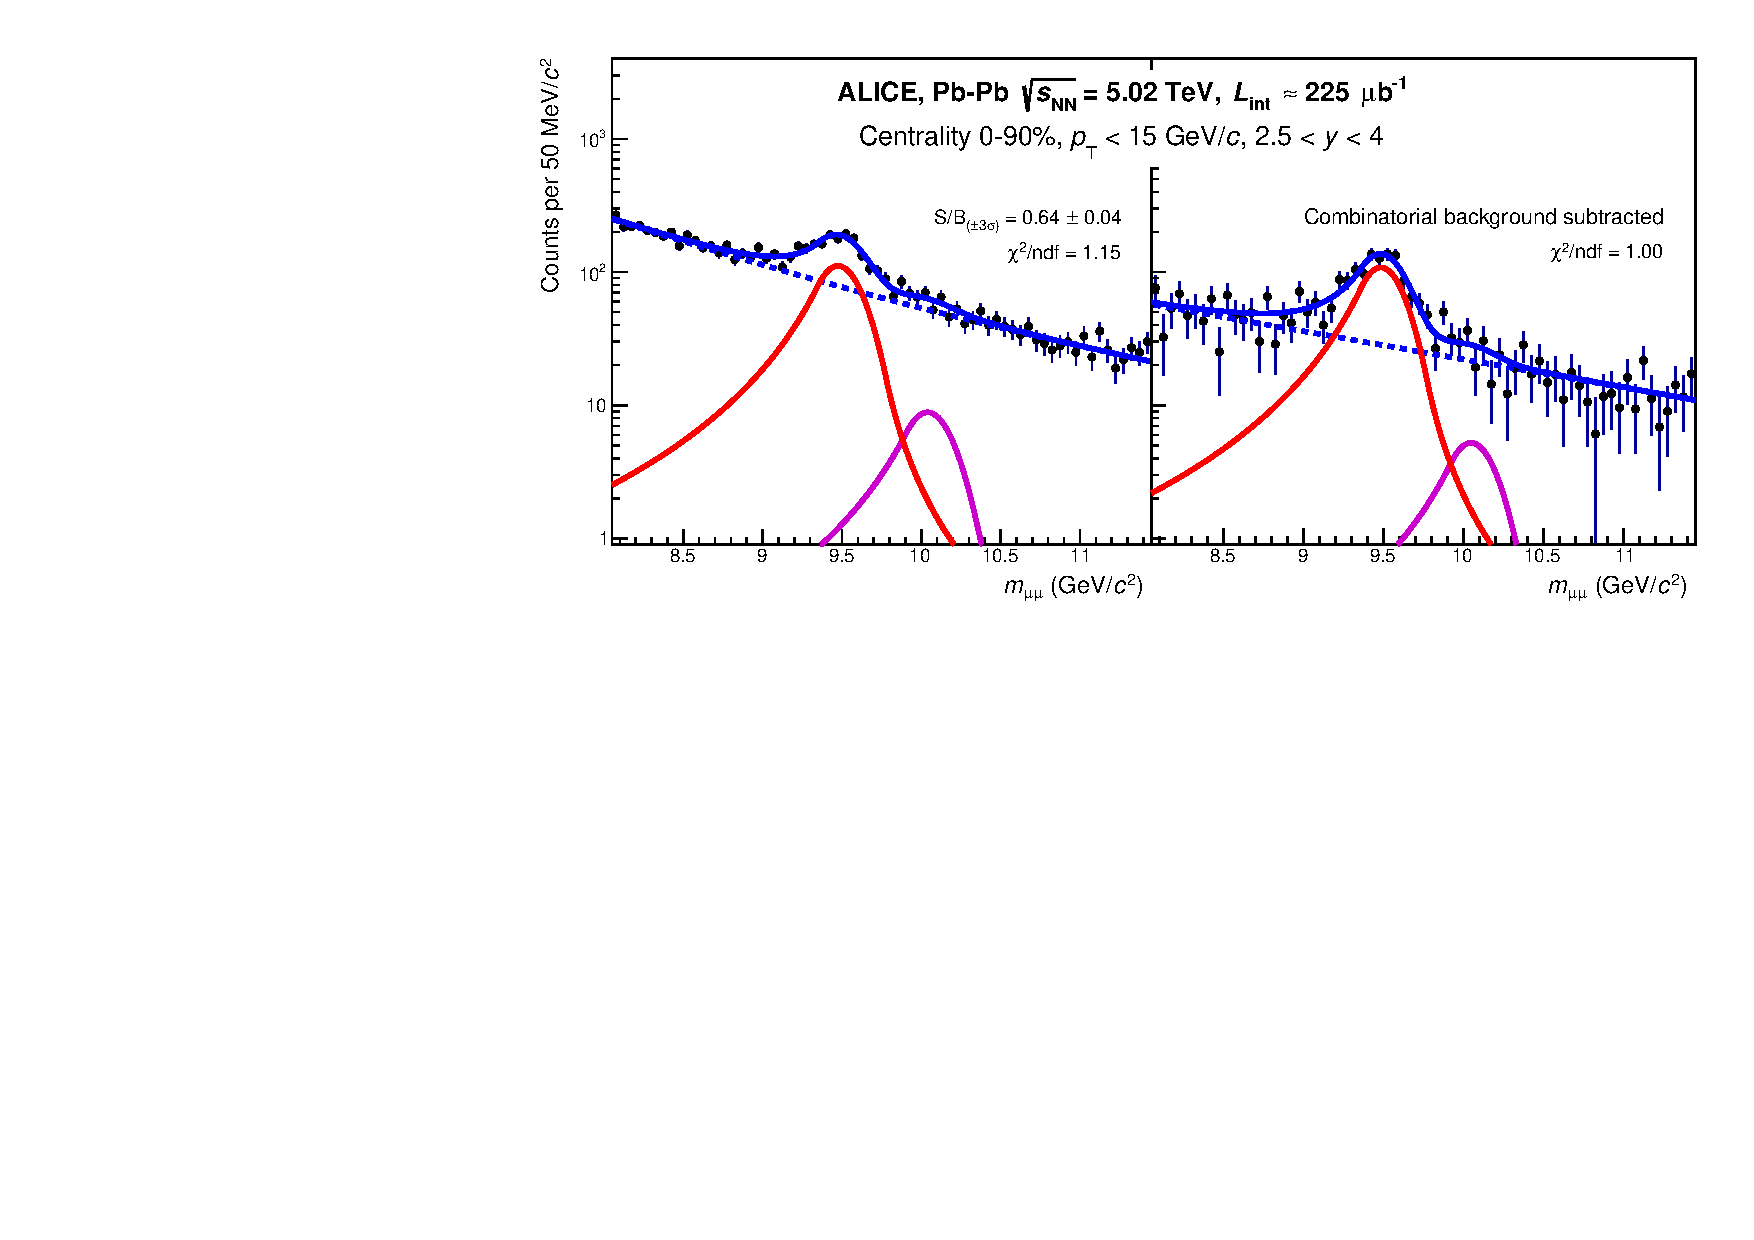
\includegraphics[width=0.8\linewidth]{Chapters/Analysis/Figs/InvMass_Upsilon_Performance_Ylog.pdf}
\caption{Dimuon invariant mass distribution (left) and combinatorial background subtracted distribution (right) in the mass region of bottomonium signals. Solid (dotted) lines correspond to signal (background) functions. The sum of the various functions is also shown as a solid line.}
\label{fig:mass_dist}
\end{center}
\end{figure}

% The analysis subject of this thesis has been performed looking at the \upsi production in the dimuon decay channel at forward rapidity.
The signal yields are evaluated by performing fits to the $\mu^+\mu^-$ invariant mass distributions.
In order to improve the purity of the dimuon sample a set of selection criteria has been applied to the muon tracks:
\begin{itemize}
\item Each track must have a transverse momentum $p_{\rm T} > 2$ GeV/$c$. 
% This cut reduces the background from $K$ and $\pi$ decays without affecting the signal of \upsi decays. 
The effect of this cut on the reconstruction efficiency is marginal;
\item Each track must exit the front absorber at a radial distance from the beam axis, $R_{abs}$, in the range $17.6 <R_{abs}< 89.5$ cm. This cut rejects tracks crossing the region of the absorber with the material of highest density, where multiple-scattering and energy- loss effects are large and affect the mass resolution;
\item A cut on product of the track momentum and the Distance of Closest Approach (DCA) between the track and the primary vertex. This additional selection reduces the contribution from fake tracks and tracks originated by beam gas collisions. This cut has been tuned to be $6\times\sigma_{pDCA}$, where $\sigma_{pDCA}$ is the resolution of this quantity.

\end{itemize}
An additional cut on the rapidity of each reconstructed $\mu$ pair is applied, rejecting the dimuons whose rapidity fell off the $2.5 < y < 4$ range, in order to remove dimuons at the edge of the acceptance region.

One of the most limiting factors for rare probes analysis is the signal-to-background ratio.
% Concerning the background affecting the bottomonium production measurements, it is mainly due to the decay in muon pairs of other species as well as to the combinatorial background caused by the decay of uncorrelated $c\bar{c}$ and $b\bar{b}$ pairs.
The background affecting the bottomonium production measurement mainly consists of $\mu^+$ and $\mu^+$ pairs from the decay of uncorrelated particles (combinatorial background) and from the correlated decay of $c\bar{c}$ and $b\bar{b}$ pairs.
% While the background can appear to be a side effect in much more abundant species, in the case of bottomonium the background needs to be treated with special care.
Two approaches are then possible to extract the yields from the fit to an invariant mass spectrum:
\begin{itemize}
\item Fit to the raw invariant mass spectrum obtained from data, where the background is modeled through a phenomenological function. In this case the fit has to be performed on the raw spectrum;
\item Estimate the contamination of the combinatorial background through the event mixing method and subtract it from the raw yields. The remaining contribution is then fitted with a suitable function to extract the signal contribution. The event-mixing technique consists in filling a dimuon invariant mass spectrum with totally uncorrelated muons ($i.e.$ from different events). Such procedure leads to an invariant mass spectrum that represents the combinatorial background of uncorrelated muons one should expect to lay under the measured dimuon invariant mass spectrum.
% Applying the event mixing method, the raw spectrum can be pre-processed, subtracting a properly scaled invariant mass spectrum which has previously been filled with dimuons composed using like-sign $\mu$ from the same collision and unlike-sign $\mu$ produced in different collisions. The ratioale of this procedure is that filling a dimuon invariant mass spectrum with totally uncorrelated muons ($i.e.$ from different events) creates an invariant mass spectrum that represents the combinatorial background one should expect when filling the signal invariant mass spectrum.
\end{itemize}

The signal component for \upsi$(1S,2S,3S)$ in the invariant mass distribution are modeled using the sum of three extended Crystal Ball (CB2) functions~\cite{ALICE-Quarkonia-signal-extraction}. 
The CB2 function consists of a Gaussian core with  power-law tails, as shown in Eq. \ref{eqn:CB2}.
The non-Gaussian tail in the low invariant mass region is due energy loss in the front absorber, while the high invariant mass one is due to residual alignment and calibration biases.
Several parameterizations of the background have been adopted.
When fitting the raw spectrum, the background has been modeled as both double exponential and double power law functions.
In case the raw spectrum has been processed with the event mixing technique, the residual background has been taken into account using a single exponential shape.

\begin{equation}\label{eqn:CB2}
f(x;N;\bar{x},\sigma,t_1,t_2,p_1,p_2) = N\cdot\begin{cases} A\cdot(B-t)^{p_1} & t<t_1,\\ -\exp\left(-\frac{1}{2}t^2\right) & t_1<t<t_2,\\C\cdot(D+t)^{p_2} & t<t_1\end{cases}
\end{equation}
\begin{equation}\label{eqn:CB2def}
\begin{aligned}
&t=\frac{x-\bar{x}}{\sigma}
\\&A=\left(\frac{p_1}{|t_1|}\right)^{p_1}\cdot\exp\left(-\frac{|t_1|^2}{2}\right)
\\&B=\frac{p_1}{t_1} - t_1
\\&C=\left(\frac{p_2}{|t_2|}\right)^{p_2}\cdot\exp\left(-\frac{|t_2|^2}{2}\right)
\\&D=\frac{p_2}{t_2} - t_2
\end{aligned}
\end{equation}

Since the signal-to-background (S/B) ratio is low in the tail regions of the extended CB functions, the CB2 tails cannot be defined using a data driven approach.
For this reason the tail parameters are fixed to values obtained from Monte-Carlo (MC) simulations. 
The mass position and the width parameters of the \upsis are left as free parameters in the fit to the integrated spectrum ($i.e.$ centrality class 0--90\%, $p_{\rm T}<15$ GeV/$c$ and $2.5 < y < 4$).
For the signal extraction as a function of centrality, the mass position  and width of the \upsis are fixed to the values obtained in the fit to the centrality-integrated (0--90\%) mass spectrum.
Some studies have been performed using the tail parameters obtained in pure MC simulation (GEANT 4) and embedded simulations (GEANT 3).
Differential tails extractions have been performed using the simulated data, then used in the fits.
Even if the tail parameters were found to be quite stable wrt $y$, \pt and centrality, the yield estimation variation has been measured to be of about $1\%$ and $3\%$ with respect to \pt and $y$ respectively.
Such uncertainty has been included in the signal extraction systematic uncertainty value.
To perform studies as a function of \pt and $y$, the mass position and the width obtained for the centrality-integrated mass spectrum are scaled according to their evolutions observed in the MC.
Due to the even smaller S/B ratio for the excited states, the mass positions of the \upsiss and \upsisss are fixed to the PDG \cite{Patrignani:2016xqp} mass differences with respect to the \upsis, and the ratio of \upsiss ($\Upsilon\text{(3S)}$) to \upsis widths is fixed to values from the MC simulation, $i.e.$ 1.03 (1.06). 
In the fit shown in Fig.~\ref{fig:mass_dist} only signals corresponding to the $\Upsilon\text{(1S)}$ and $\Upsilon\text{(2S)}$ are visible, since the $\Upsilon\text{(3S)}$ contribution turns out to be compatible with zero events.
 
%%%%%%%%%%%%%%%%%%%%%%%%%%%%%%%%%%%%%%%%%%%%%%%%
\section{Acceptance and efficiency correction}

\begin{figure}[htp]

\centering
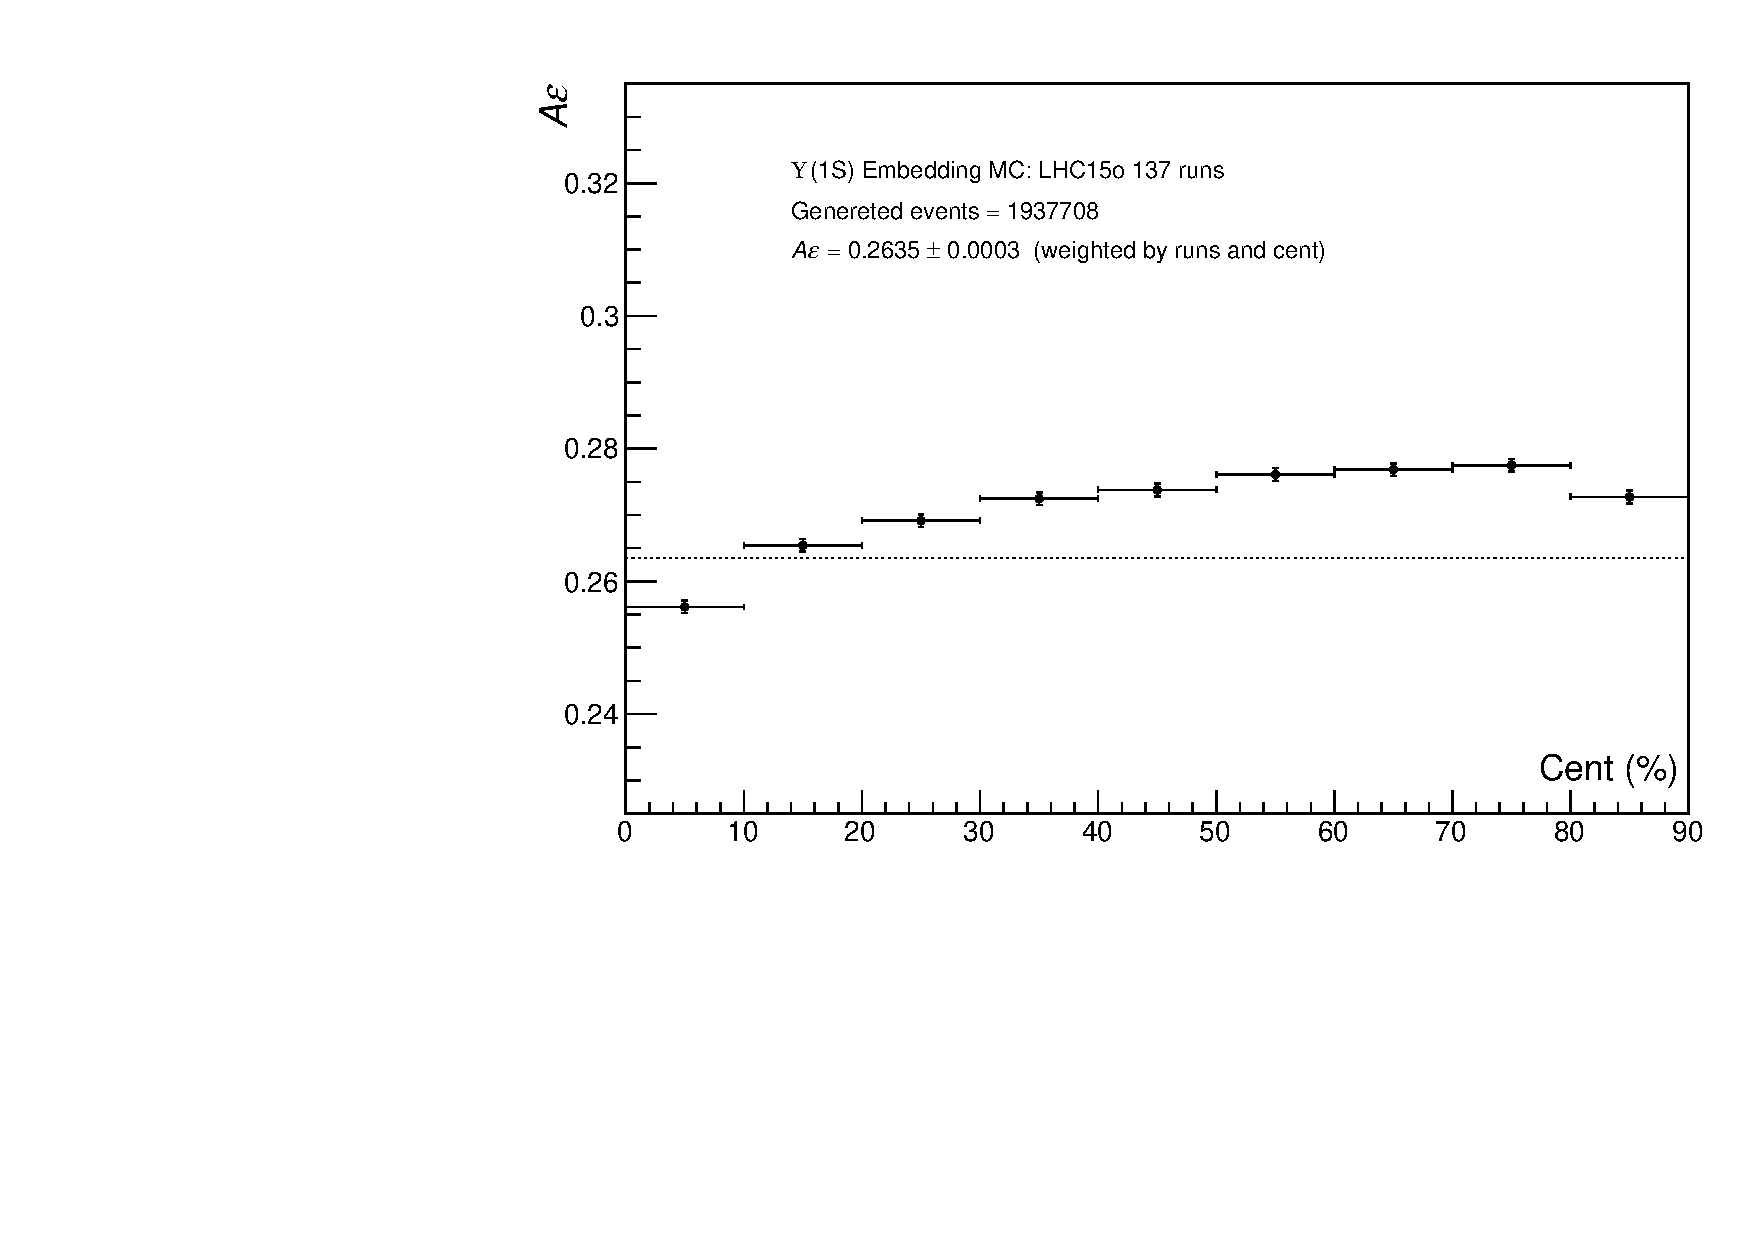
\includegraphics[width=.5\textwidth]{Chapters/Analysis/Figs/Axe/AccEffvsCent.pdf}\hfill
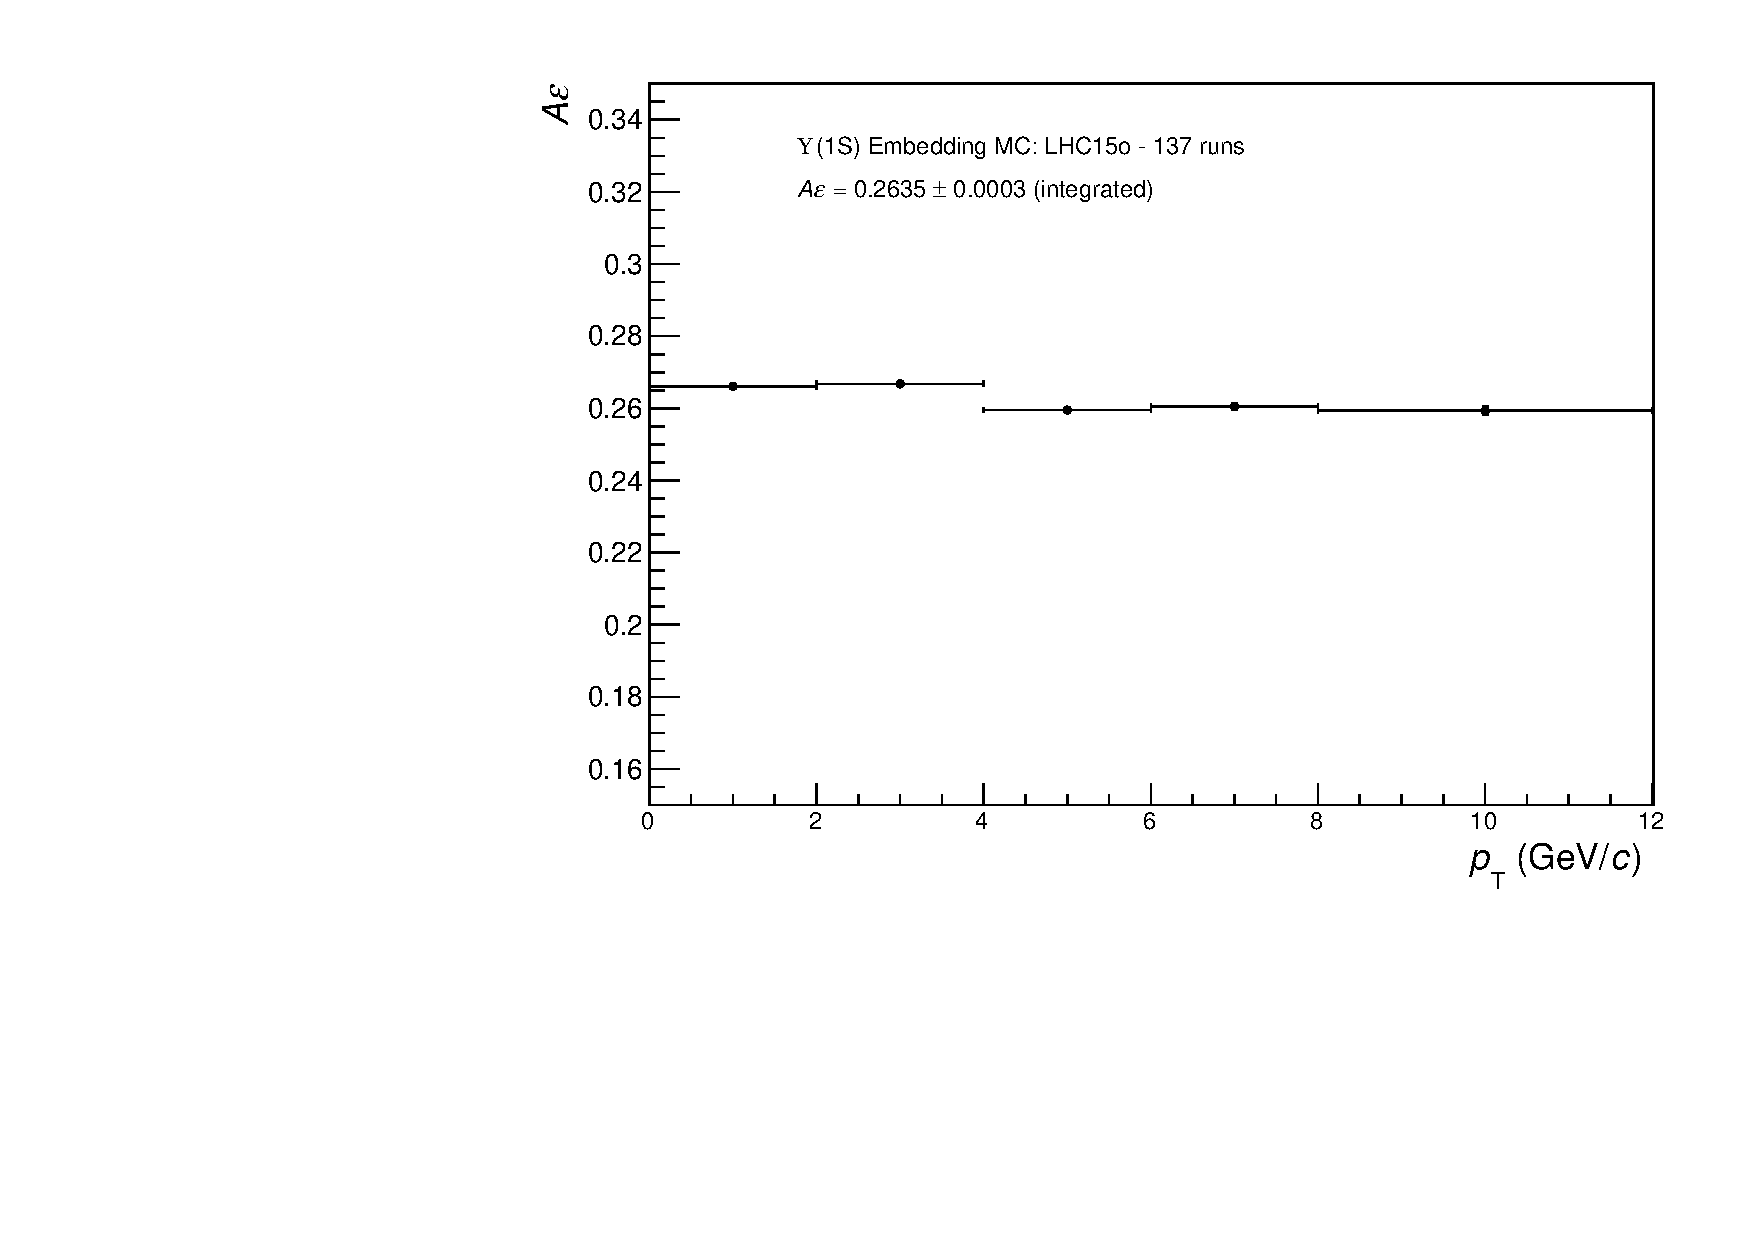
\includegraphics[width=.5\textwidth]{Chapters/Analysis/Figs/Axe/AccEffvsPt.pdf}\hfill
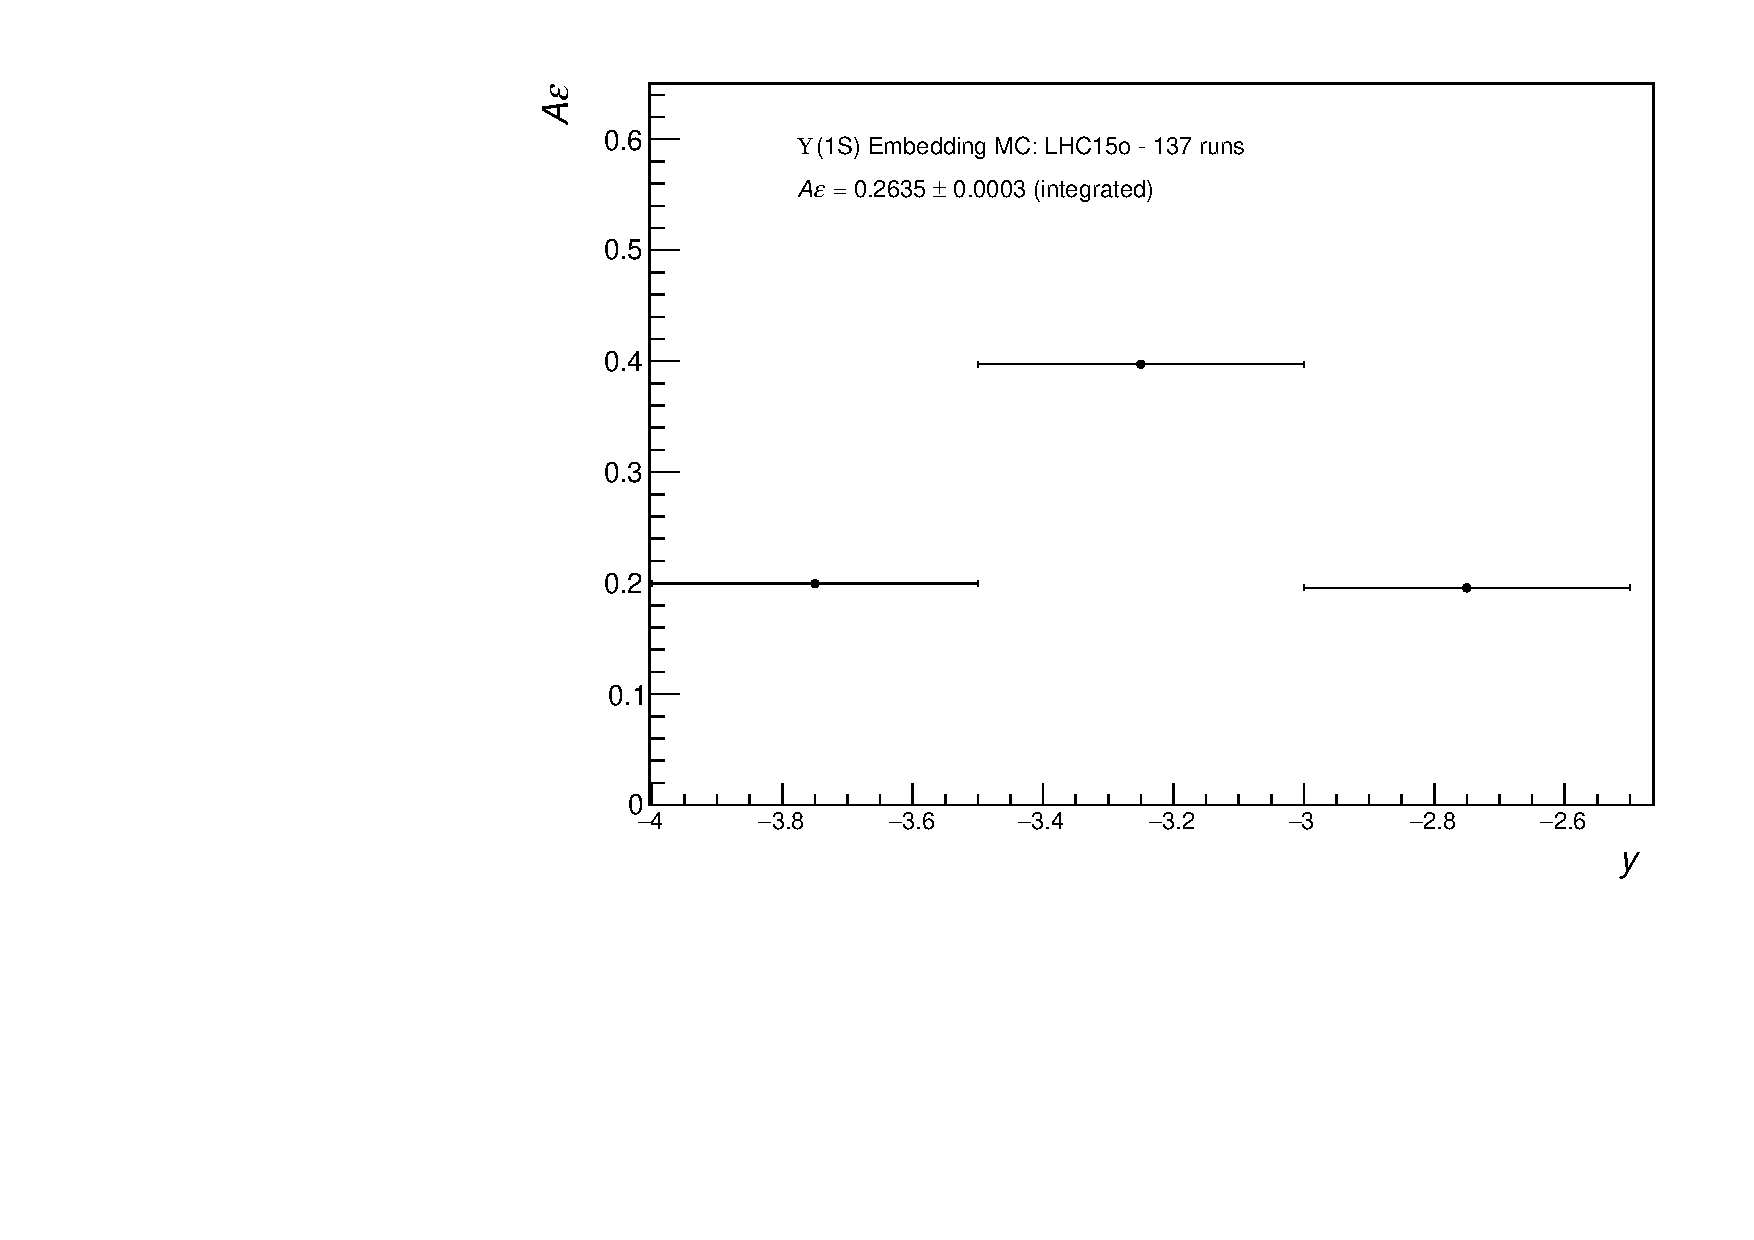
\includegraphics[width=.5\textwidth]{Chapters/Analysis/Figs/Axe/AccEffvsY.pdf}

\caption{$A\times\epsilon$ as a function of centrality (left), \pt (center), and $y$ (right). The values have been computed using embedded Monte Carlo events.}
\label{fig:Axe}

\end{figure}

% One of the ingredients appearing in the nuclear modification factor definition reported in equation \ref{eqn:raa} is the $A\times\epsilon$ correction.
The extracted number of Upsilon must be corrected by the product of the acceptance and efficiency of the detector ($A\times\epsilon$).
This correction is needed to turn the raw spectrum into one that contains physics information.
Acceptance and efficiency of each detector are evaluated through custom MC simulations.
In particular the so called "embedded" simulations are used for this studies.
In such MC simulations, the generated \upsi is embedded in a real recorded event.
This allows one to test the efficiency of detection of the simulated signal in a real event, with the full multiplicity observed in real data.
This simulation can be used for efficiency studies as well as for the acceptance ones.
% Two kinds of simulations are performed:
% \begin{itemize}
% \item Standard MC simulations: the whole event is generated by the generator and then reconstructed. The overall multiplicity is limited and this kind of simulations is useful for acceptance studies;
% \item Embedded MC simulations: the generated \upsi is embedded in a real recorded event.  This allows to test the efficiency of detection of the simulated signal in a real event, with the full multiplicity observed in real data. This simulation can be used for efficiency studies.
% \end{itemize}
Some inputs have to be provided to the MC generator.
The simulation input consists of a parameterization of the bottomonium \pt and $y$ distribution obtained by interpolating existing $pp$ measurements \cite{Acosta:2001gv,LHCb:2012aa,Khachatryan:2010zg} with the procedure described in \cite{Bossu:2011qe}.
% In particular the \pt and $y$ distributions of the generated \upsi are obtained from existing $pp$ measurements ~\cite{Acosta:2001gv,LHCb:2012aa,Khachatryan:2010zg} using the interpolation and extrapolation procedure described in~\cite{Bossu:2011qe}. 
The EKS98 nuclear shadowing parameterization~\cite{Eskola:1998df} is used to include an estimate of CNM effects.
Since available data favor a small or null polarization for $\Upsilon$(1S)~\cite{Abazov:2008aa,CDF:2011ag,Chatrchyan:2012woa}, an unpolarized production was assumed. 
The variations of the performance of the muon tracker and muon trigger systems throughout the data-taking period as well as the residual misalignment of the tracking chambers are taken into account in the simulation.

The $A\times\epsilon$ values, for the range $p_{\rm T} < 15$ GeV/$c$, $2.5 < y < 4$ and the 0--90\% centrality class are $0.263$ and $0.264$ for the \upsis and \upsiss, respectively. 
A decrease of $0.02$ is observed in  $A\times\epsilon$ for the 0--10\% central collisions with respect to the 50--90\%. 
This effect is due to a limitation of the Muon Trigger related to the higher occupancy in the most central events.
In fact the Muon Trigger LBs can provide only one tracklet each, hence if two muons cross the same LB only one of the two particles is correctly reconstructed.
Further details are given in section \ref{MTR_tagging}.
Differential studies of $A\times\epsilon$ are presented in the plots reported in figure \ref{fig:Axe}.

\section{Reference pp cross section}
\label{sec:ppxsection}
The evaluation of \raa requires to divide the yield measured in Pb-Pb collisions by the cross-section measured in $pp$ collisions at the same energy.
The statistics of the ALICE measurement at $\sqrt{s}=5.02$ in $pp$ collisions was not sufficient to provide an estimate of the \upsi cross section \cite{Adam:2016rdg}.
For this reason the reference proton-proton cross sections, for \upsis and \upsiss production, have been computed by means of an interpolation procedure described below.
The energy interpolation for the \upsi cross section, as a function of rapidity and for the \pt and $y$ integrated result, uses the measurements of \upsi production cross sections in \pp collisions at $\sqrt{s}=7$ and $8$ \rm{TeV} by ALICE \cite{Abelev:2014qha,Adam:2015rta} and at $\sqrt{s}=2.76, 7$ and $8$ \rm{TeV} by LHCb \cite{Aaij:2014nwa,Aaij:2015awa}. 
In order to obtain the reference cross section in the same \pt and $y$ bins as the ones used for the analysis, measurements from LHCb in finer \pt and $y$ bins have been combined.
The obtained values for different \pt intervals, coming from LHCb data only, are reported in tables \ref{table:LHCbData276}, \ref{table:LHCbData7} and \ref{table:LHCbData8}.
The obtained values in different $y$ bins, obtained combining both ALICE and LHCb results, are reported in tables \ref{table:LHCbY1sData276}, \ref{table:LHCbY1sData7}, \ref{table:ALICEY1sData7}, \ref{table:LHCbY1sData8} and \ref{table:ALICEY1sData8}.

\begin{table}[htp]
\begin{center}
\begin{tabular}{|c||c|c|c|c|c|c|}
  \hline
  \multicolumn{7}{|c|}{$\sqrt{s_{pp}}=$ 2.76 TeV, $2.5<y<4.0$}\\
  \hline
  $p_\mathrm{T}$ bin & $\sigma_{pp}^{\Upsilon\rightarrow \mu^{+}\mu^{\--}} $ & Stat. & uncorr. Syst. & fully corr. Syst. & Total & Relative \\
  \hline
  GeV/c & \multicolumn{5}{c|}{pb} & $\%$ \\
  \hline
  $0.0 < p_\mathrm{T} < 2.0 $ & 154,2 & 12,6 & 0,0 & 6,6 & 14,2 & 9,2 \\
  \hline
  $2.0 < p_\mathrm{T} < 4.0 $& 192,6 & 12,8 & 0,0	 & 9,6 & 16,0 & 8,3\\
  \hline
  $4.0 < p_\mathrm{T} < 6.0 $& 166,2 & 13,8 & 0,0	 & 7,8 & 15,9 & 9,5\\
  \hline
  $6.0 < p_\mathrm{T} < 15.0 $& 153,0 & 12,4	 & 0,0 & 6,6 & 14,0 & 9,2\\
  \hline
\end{tabular}
\caption{Reference cross sections and corresponding uncertainties in different $p_\mathrm{T}$ intervals. $\sigma_{pp}^{\Upsilon\rightarrow \mu^{+}\mu^{\--}} $ values and uncertainties as obtained using LHCb $pp$ data at $\sqrt{s_{pp}}=$ 2.76 TeV.}\label{table:LHCbData276}
\end{center}
\end{table}

\begin{table}[htp]
\begin{center}
\begin{tabular}{|c||c|c|c|c|c|c|}
  \hline
  \multicolumn{7}{|c|}{$\sqrt{s_{pp}}=$ 7 TeV, $2.5<y<4.0$}\\
  \hline
  $p_\mathrm{T}$ bin & $\sigma_{pp}^{\Upsilon\rightarrow \mu^{+}\mu^{\--}} $ & Stat. & uncorr. Syst. & fully corr. Syst. & Total & Relative \\
  \hline
  GeV/c & \multicolumn{5}{c|}{pb} & $\%$ \\
  \hline
  $0.0 < p_\mathrm{T} < 2.0 $ & 278,750 & 0,917 & 1,078 & 8,641 & 8,756 & 3,141 \\
  \hline
  $2.0 < p_\mathrm{T} < 4.0 $& 497,600 & 1,311 & 1,105 & 15,426 & 15,521 & 3,119 \\
  \hline
  $4.0 < p_\mathrm{T} < 6.0 $& 385,600 & 1,068 & 1,054 & 11,954 & 12,047 & 3,124 \\
  \hline
  $6.0 < p_\mathrm{T} < 15.0 $& 473,720 & 1,197 & 0,936 & 14,685 & 14,764 & 3,117 \\
  \hline
\end{tabular}
\caption{Reference cross sections and corresponding uncertainties in different $p_\mathrm{T}$ intervals. $\sigma_{pp}^{\Upsilon\rightarrow \mu^{+}\mu^{\--}} $ values and uncertainties as obtained using LHCb $pp$ data at $\sqrt{s_{pp}}=$ 7 TeV.}\label{table:LHCbData7}
\end{center}
\end{table}

\begin{table}[htp]
\begin{center}
\begin{tabular}{|c||c|c|c|c|c|c|}
  \hline
  \multicolumn{7}{|c|}{$\sqrt{s_{pp}}=$ 8 TeV, $2.5<y<4.0$}\\
  \hline
  $p_\mathrm{T}$ bin & $\sigma_{pp}^{\Upsilon\rightarrow \mu^{+}\mu^{\--}} $ & Stat. & uncorr. Syst. & fully corr. Syst. & Total & $\%$ \\
  \hline
  GeV/c & \multicolumn{5}{c|}{pb} & $\%$ \\
  \hline
  $0.0 < p_\mathrm{T} < 2.0 $ & 337.680 & 0.811 & 0.967 & 9.455 & 9.539 & 2.825 \\
  \hline
  $2.0 < p_\mathrm{T} < 4.0 $& 610.400 & 1.068 & 1.367 & 17.091 & 17.179 & 2.814 \\
  \hline
  $4.0 < p_\mathrm{T} < 6.0 $& 481.000 & 0.906 & 1.010 & 13.468 & 13.536 & 2.814 \\
  \hline
  $6.0 < p_\mathrm{T} < 15.0 $& 609.970 & 1.022 & 0.905 & 17.079 & 17.134 & 2.809 \\
  \hline
\end{tabular}
\caption{Reference cross sections and corresponding uncertainties in different $p_\mathrm{T}$ intervals. $\sigma_{pp}^{\Upsilon\rightarrow \mu^{+}\mu^{\--}} $ values and uncertainties as obtained using LHCb $pp$ data at $\sqrt{s_{pp}}=$ 8 TeV.}\label{table:LHCbData8}
\end{center}
\end{table}

\begin{table}[!tp]
\begin{center}
\begin{tabular}{|c||c|c|c|c|c|c|}
  \hline
  \multicolumn{7}{|c|}{$\sqrt{s_{pp}}=$ 2.76 TeV, $0<p_\mathrm{T}<15$}\\
  \hline
  $y$ bin & $d(\sigma_{pp}^{\Upsilon\rightarrow \mu^{+}\mu^{\--}})/dy $ & Stat. & uncorr. Syst. & fully corr. Syst. & Total & $\%$ \\
  \hline
  GeV/c & \multicolumn{5}{c|}{pb} & $\%$ \\
  \hline
  $2.5 < y < 3.0 $ & 642 & 36 & 0 & 24 & 43 & 7 \\
  \hline
  $3.0 < y < 3.5 $& 454 & 26 & 0 & 16 & 31 & 7 \\
  \hline
  $3.5 < y < 4.0 $& 248 & 22 & 0 & 10 & 24 & 10 \\
  \hline
  $2.5 < y < 4.0 $& 448 & 17 & 0 & 16 & 24 & 5 \\
  \hline
\end{tabular}
\caption{$y$ bins $d(\sigma_{pp}^{\Upsilon\rightarrow \mu^{+}\mu^{\--}})/dy $ values and uncertainties as obtained using LHCb $pp$ data at $\sqrt{s_{pp}}=$ 2,76 TeV.}\label{table:LHCbY1sData276}
\end{center}
\end{table}

\begin{table}[!tp]
\begin{center}
\begin{tabular}{|c||c|c|c|c|c|c|}
  \hline
  \multicolumn{7}{|c|}{$\sqrt{s_{pp}}=$ 7 TeV, $0<p_\mathrm{T}<15$}\\
  \hline
  $y$ bin & $d(\sigma_{pp}^{\Upsilon\rightarrow \mu^{+}\mu^{\--}})/dy $ & Stat. & uncorr. Syst. & fully corr. Syst. & Total & $\%$ \\
  \hline
  GeV/c & \multicolumn{5}{c|}{pb} & $\%$ \\
  \hline
  $2.5 < y < 3.0 $ & 1291.40 & 2.96 & 2.08 & 40.20 & 40.36 & 3.1 \\
  \hline
  $3.0 < y < 3.5 $& 1116.58 & 2.48 & 2.04 & 34.76 & 34.91 & 3.1 \\
  \hline
  $3.5 < y < 4.0 $& 863.36 & 2.40 & 2.98 & 27.04 & 27.31 & 3.2 \\
  \hline
  $2.5 < y < 4.0 $& 1090.45 & 4.55 & 4.17 & 33.80 & 34.36 & 3.2 \\
  \hline
\end{tabular}
\caption{$y$ bins $d(\sigma_{pp}^{\Upsilon\rightarrow \mu^{+}\mu^{\--}})/dy $ values and uncertainties as obtained using LHCb $pp$ data at $\sqrt{s_{pp}}=$ 7 TeV.}\label{table:LHCbY1sData7}
\end{center}
\end{table}

\begin{table}[!tp]
\begin{center}
\begin{tabular}{|c||c|c|c|c|c|c|}
  \hline
  \multicolumn{7}{|c|}{$\sqrt{s_{pp}}=$ 8 TeV, $0<p_\mathrm{T}<15$}\\
  \hline
  $y$ bin & $d(\sigma_{pp}^{\Upsilon\rightarrow \mu^{+}\mu^{\--}})/dy $ & Stat. & uncorr. Syst. & fully corr. Syst. & Total & $\%$ \\
  \hline
  GeV/c & \multicolumn{5}{c|}{pb} & $\%$ \\
  \hline
  $2.5 < y < 3.0 $ & 1659.32 & 2.50 & 2.44 & 46.60 & 46.73 & 2.8 \\
  \hline
  $3.0 < y < 3.5 $& 1370.82 & 2.04 & 2.66 & 38.52 & 38.67 & 2.8 \\
  \hline
  $3.5 < y < 4.0 $& 1047.96 & 2.06 & 2.34 & 29.50 & 29.66 & 2.8 \\
  \hline
  $2.5 < y < 4.0 $& 1359.37 & 3.83 & 4.30 & 38.06 & 38.50 & 2.8 \\
  \hline
\end{tabular}
\caption{$y$ bins $d(\sigma_{pp}^{\Upsilon\rightarrow \mu^{+}\mu^{\--}})/dy $ values and uncertainties as obtained using LHCb $pp$ data at $\sqrt{s_{pp}}=$ 8 TeV.}\label{table:LHCbY1sData8}
\end{center}
\end{table}

\begin{table}[!tp]
\begin{center}
\begin{tabular}{|c||c|c|c|c|c|c|}
  \hline
  \multicolumn{7}{|c|}{$\sqrt{s_{pp}}=$ 7 TeV, $0<p_\mathrm{T}<12$}\\
  \hline
  $y$ bin & $d(\sigma_{pp}^{\Upsilon\rightarrow \mu^{+}\mu^{\--}})/dy $ & Stat. & uncorr. Syst. & fully corr. Syst. & Total & $\%$ \\
  \hline
  GeV/c & \multicolumn{5}{c|}{pb} & $\%$ \\
  \hline
  $2.5 < y < 3.0 $ & 1158.16 & 183.52 & 151.52 & 58.03 & 244.81 & 21.1 \\
  \hline
  $3.0 < y < 3.5 $& 944.88 & 143.84 & 163.68 & 47.37 & 222.99 & 23.6 \\
  \hline
  $3.5 < y < 4.0 $& 607.60 & 124.00 & 81.84 & 30.50 & 151.67 & 25.0 \\
  \hline
  $2.5 < y < 4.0 $& 896.11 & 82.67 & 110.77 & 44.81 & 145.30 & 17.2 \\
  \hline
\end{tabular}
\caption{$y$ bins $d(\sigma_{pp}^{\Upsilon\rightarrow \mu^{+}\mu^{\--}})/dy $ values and uncertainties as obtained using ALICE $pp$ data at $\sqrt{s_{pp}}=$ 7 TeV.}\label{table:ALICEY1sData7}
\end{center}
\end{table}

\begin{table}[!tp]
\begin{center}
\begin{tabular}{|c||c|c|c|c|c|c|}
  \hline
  \multicolumn{7}{|c|}{$\sqrt{s_{pp}}=$ 8 TeV, $0<p_\mathrm{T}<12$}\\
  \hline
  $y$ bin & $d(\sigma_{pp}^{\Upsilon\rightarrow \mu^{+}\mu^{\--}})/dy $ & Stat. & uncorr. Syst. & fully corr. Syst. & Total & $\%$ \\
  \hline
  GeV/c & \multicolumn{5}{c|}{pb} & $\%$ \\
  \hline
  $2.5 < y < 3.0 $ & 1669.04 & 270.32 & 143.84 & 83.45 & 317.38 & 19.0 \\
  \hline
  $3.0 < y < 3.5 $& 1173.04 & 136.40 & 91.76 & 58.65 & 174.54 & 14.9 \\
  \hline
  $3.5 < y < 4.0 $& 806.00 & 161.20 & 89.28 & 40.30 & 188.63 & 23.4 \\
  \hline
  $2.5 < y < 4.0 $& 1173.87 & 99.20 & 115.73 & 58.69 & 163.34 & 13.9 \\
  \hline
\end{tabular}
\caption{$y$ bins $d(\sigma_{pp}^{\Upsilon\rightarrow \mu^{+}\mu^{\--}})/dy $ values and uncertainties as obtained using ALICE $pp$ data at $\sqrt{s_{pp}}=$ 8 TeV.}\label{table:ALICEY1sData8}
\end{center}
\end{table}

The energy interpolation is performed fitting the experimental data using the empirical functions listed below:
\begin{itemize}
    \item Linear function: $p_0+p_1\cdot\sqrt{s}$
    \item Parabola: $p_0\cdot\sqrt{s}+p_1\cdot(\sqrt{s})^2$
    \item Positive exponential: $p_0\cdot\sqrt{s}\cdot e^{\frac{\sqrt{s}}{p_1}}$
    \item Negative exponential: $p_0\cdot(1-e^{\frac{-\sqrt{s}}{p_1}})$
    \item Power law: $p_0\cdot(\sqrt{s})^{p_1}$
\end{itemize}
The requirement for such functions is to be able to intercept the origin of the axes.
This choice is driven by the convincing assumption that at $\sqrt{s}=0$ \rm{TeV}  the cross-section drops to $0$.
% In addition to the functions satisfying this requirement, representing the first order Taylor expansion of any other functional form, a straight line has been added to the set of interpolating functions.
The energy interpolation for the \upsis cross section as a function of \pt is based on LHCb measurements only, since the  \pt coverage of the results of this analysis ($p_{\rm T} < 15$ GeV/$c$) is more extended than that of the corresponding ALICE $pp$ data ($p_{\rm T} < 12$ GeV/$c$).
The plots representing the data points, the interpolation functions and the interpolated values are shown in figure \ref{fig:sigmapp}.

\begin{figure}[!b]
\begin{center}
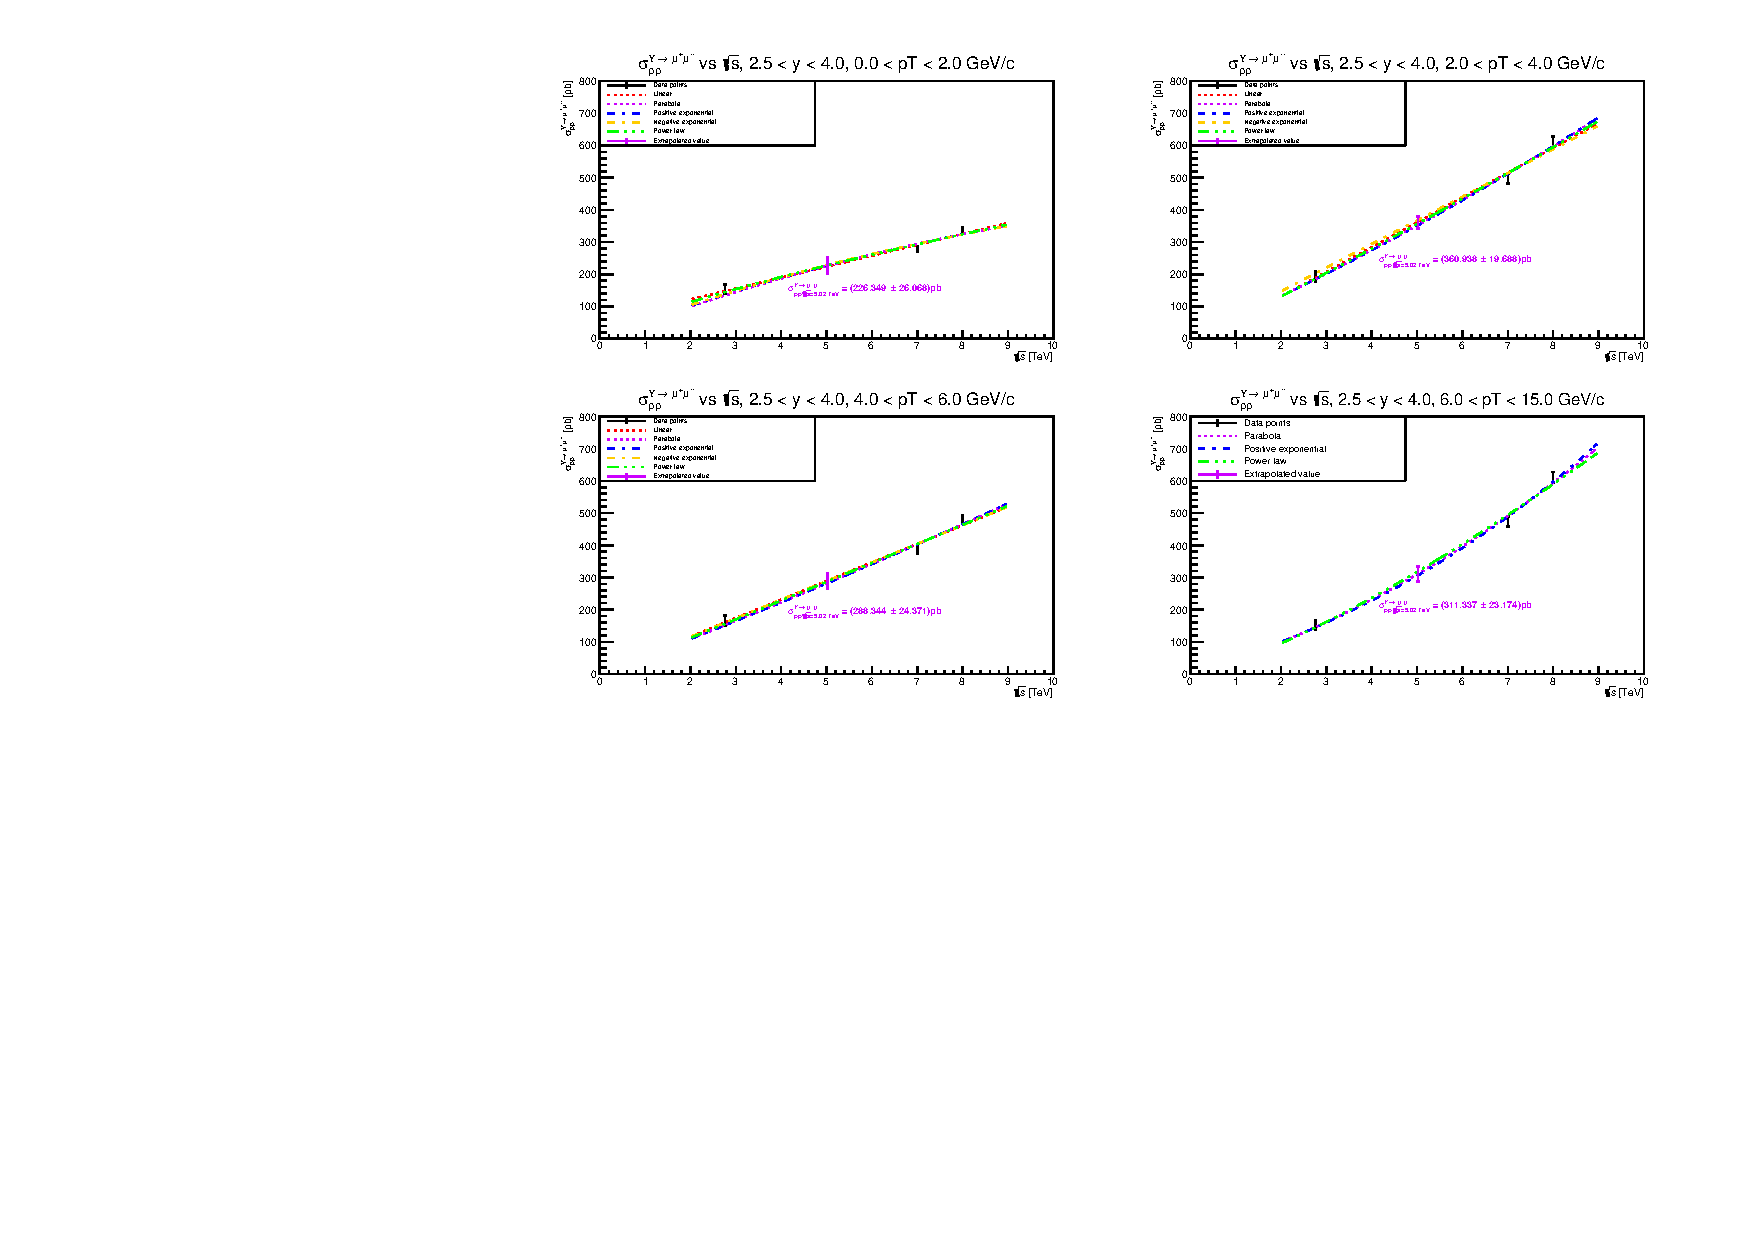
\includegraphics[width=0.95\linewidth]{Chapters/Analysis/Figs/sigmapp_vs_pt.pdf}
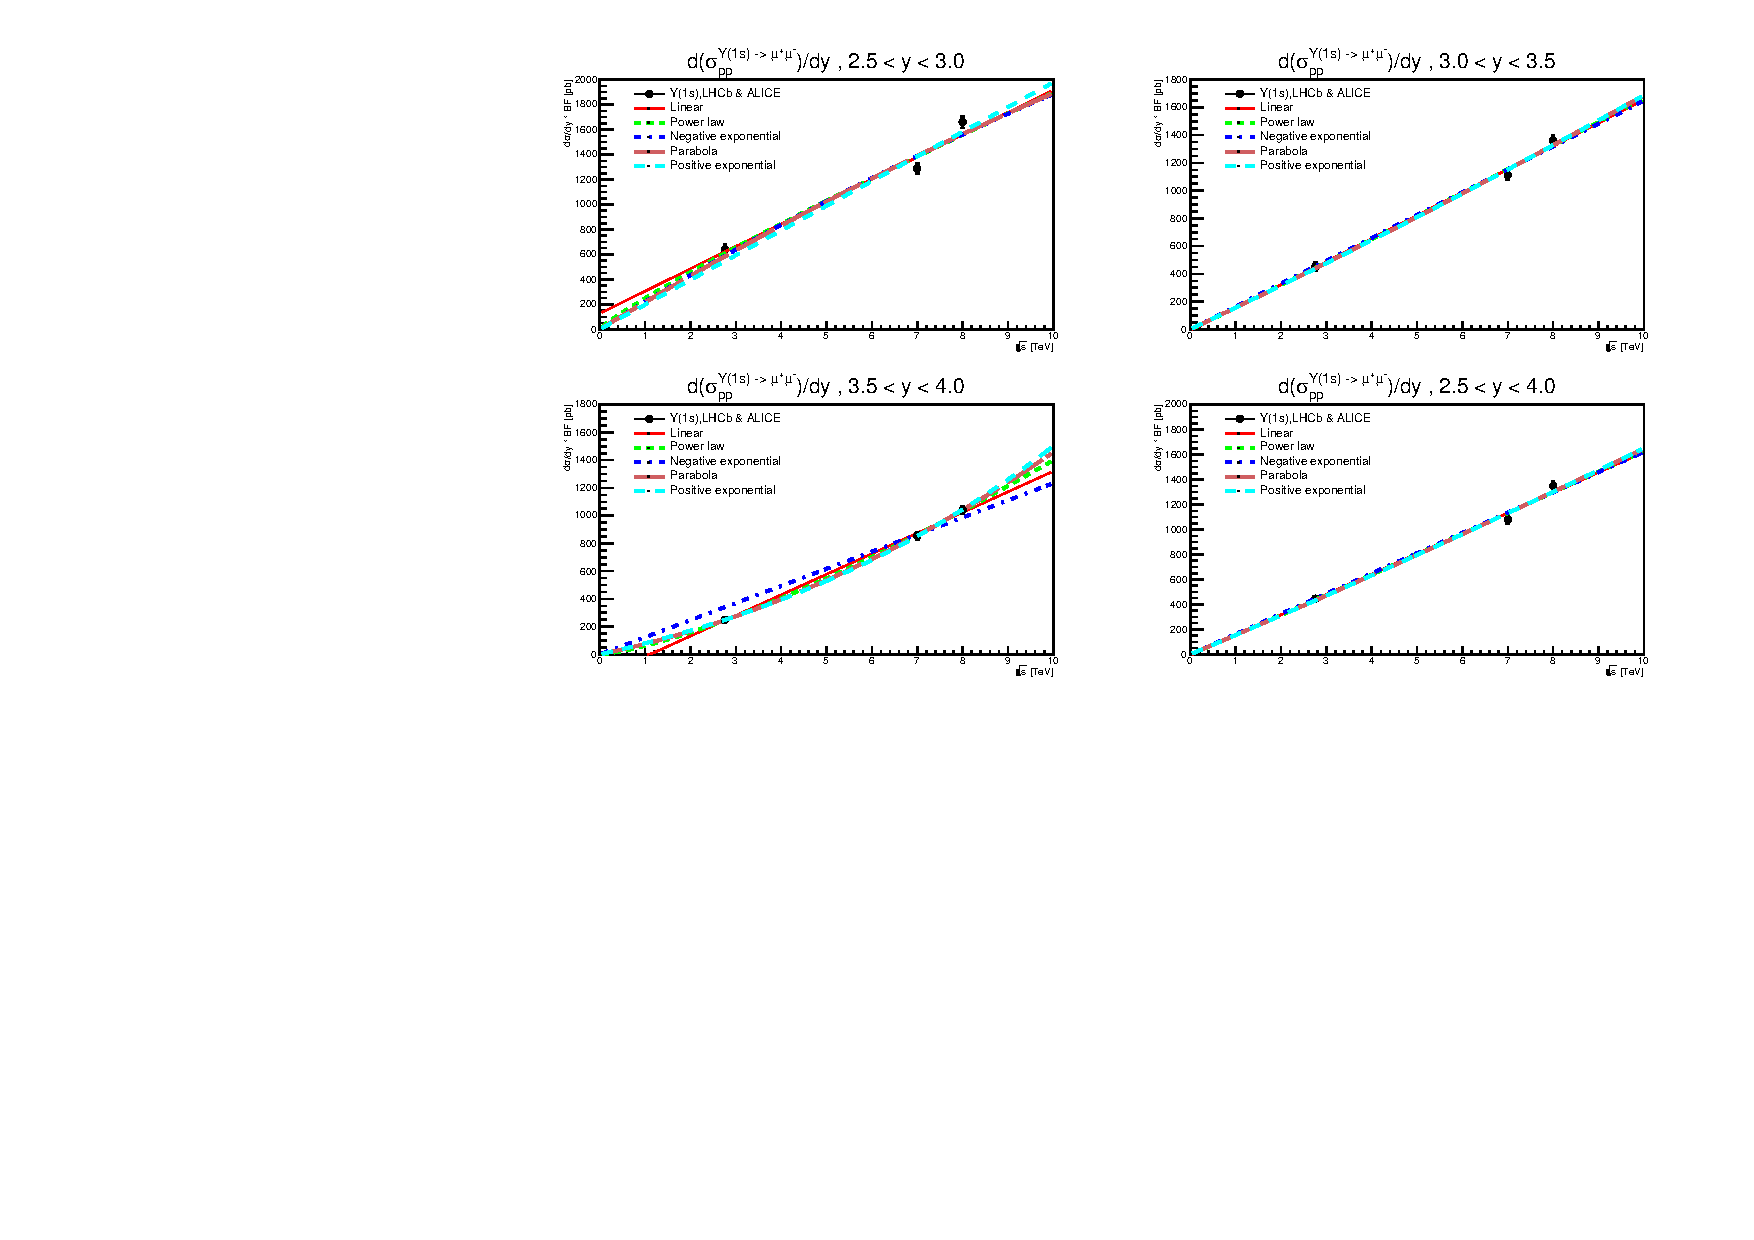
\includegraphics[width=0.95\linewidth]{Chapters/Analysis/Figs/sigmapp_vs_y.pdf}
\caption{Interpolation of reference $\sigma_{pp}$ in \pt (top 4 graphs) and $y$ (bottom 4 graphs) bins. The measured points are reported with an error bar that is the quadratic sum of the statistical and systematic uncertainties.}
\label{fig:sigmapp}
\end{center}
\end{figure}

The final cross section value is the weighted average of the whole set of interpolated values.
The total uncertainty on the interpolated $pp$ cross-section corresponds to the quadratic sum of two terms. 
One term represents the statistical uncertainty and reflects the uncertainties on the data samples used in the interpolation procedure.
% This term is the uncertainty on the average of the interpolated values using the whole set of functions and theoretical models.
The second term represents the systematic uncertainty related to the interpolation procedure itself.
It corresponds to the maximum spread between the final cross section value and each single interpolation.
The numerical values obtained from the interpolation procedure are summarized in Table~\ref{tab:ref_cs_pp} for the various kinematic ranges used in the analysis.
The result of the interpolation procedure gives ${\rm BR}_{\Upsilon\text{(1S)} \rightarrow \mu^{+} \mu^{-}} \cdot \sigma^{\rm\Upsilon({\rm 1S})}_{\rm pp}=1221\pm77\text{(tot)}$~pb and ${\rm BR}_{\Upsilon\text{(2S)} \rightarrow \mu^{+} \mu^{-}} \cdot \sigma^{\rm\Upsilon({\rm 2S})}_{\rm pp}=302\pm23\text{(tot)}$~pb assuming unpolarized quarkonia and integrating over the ranges $2.5 < y < 4$ and $p_{\rm T} < 15\ GeV/c$.
% These values differ from the sum of the differential values reported in \ref{tab:ref_cs_pp}.
% The integrated values are 

\begin{table}[!t]
\centering
\begin{tabular}{| c | c | c |}
\hline
\pt (GeV/$c$) & $y$ & ${\rm BR}_{\Upsilon\text{(1S)} \rightarrow \mu^{+} \mu^{-}} \cdot \sigma_{\rm pp}^{\Upsilon{\rm (1S)}}$ (pb) \tabularnewline
\hline 
{[}0-2{]} & \multirow{4}{*}{{[}2.5-4{]}} & $226 \pm 26$\tabularnewline
%\cline{1-1} \cline{3-3} 
{[}2-4{]} &  & $361 \pm 20$\tabularnewline
%\cline{1-1} \cline{3-3} 
{[}4-6{]} &  & $288 \pm 24$\tabularnewline
%\cline{1-1} \cline{3-3} 
{[}6-15{]} &  & $311 \pm 23$\tabularnewline
\hline 
\multirow{3}{*}{{[}0-15{]}} & {[}2.5-3{]} & $ 506 \pm 57 $\tabularnewline
%\cline{2-3} 
 & {[}3-3.5{]} & $ 415 \pm 28 $\tabularnewline
%\cline{2-3} 
 & {[}3.5-4{]} & $ 288 \pm 24$\tabularnewline
\hline 
\end{tabular}
\caption{\label{tab:ref_cs_pp} The interpolated branching ratio times cross section of \upsis for the \pt and $y$ bins under study.}
\end{table}

It should be noted that the integrals of the interpolated  $p_{\mathrm{T}}$-differential and $y$-differential  cross sections differ by at most $\approx3\%$ from the interpolated integrated cross sections. 
This indicates a good consistency of the interpolation procedure across various kinematical ranges, also considering that the uncertainties on the obtained cross sections are not completely correlated.

% % %%%%%%%%%%%%%%%%%%%%%%%%%%%%%%%%%%%%%%%%%%%%%%%%
\section{Uncertainties}\label{subsec:syst_uncert}

The systematic uncertainty on \raa has several contributions related to the various ingredients which constitute the nuclear modification definition in equation \ref{eqn:raa}.
% Several procedures have been performed to obtain such ingredients and the systematic uncertainty contribution of each of these procedures has to be evaluated and quoted alongside the final result.
The estimation of the systematic uncertainties will be detailed in the following.

The systematic uncertainty on the signal extraction is evaluated by considering the variations in the signal counts when using various functions for the description of the background for the invariant mass distribution, as well as adopting two fitting ranges, $i.e.$ $(7-14)$ GeV/$c^2$ and $(7.5-14.5)$ GeV/$c^2$.
As it has already been mentioned, the signal extraction procedure can be performed either on the raw mass spectrum or on the mass spectrum with applied event mixing subtraction.
In both cases, the resulting distribution is fitted with the sum of three extended CB and a function to account for the residual background.
The extended CB tail parameters have been varied using estimates provided by two MC transport models: GEANT4~\cite{Agostinelli:2002hh} and GEANT3~\cite{Brun:1082634}. 
Due to lack of statistics for the higher mass bottomonium resonances, the mass position and width of the \upsiss and \upsisss have been fixed to the \upsis position and width obtained from the fit, using the ratio obtained from the PDG as scaling factor.
To take in account for the statistical uncertainty on such choice, the ratio of \upsiss ($\Upsilon\text{(3S)}$) to \upsis widths is varied from 1 (1) to 1.06 (1.12).
In the centrality, \pt or $y$ differential studies, the mass position and width are also varied, by an amount which corresponds to the uncertainties on the mass position and the width returned by the fit to the integrated invariant mass spectrum. 
The central values of $N^{\Upsilon}$ and their statistical uncertainties are obtained by taking the weighted average of $N^{\Upsilon}$ and of the corresponding statistical uncertainties from the various fits.
The systematic uncertainties are estimated as the root mean square of the distribution of $N^{\Upsilon}$ obtained from the various fits.

As already reported, a cut of $p_{\rm T} > 2$ GeV/$c$ on single muons has been applied to filter out the contribution of muons from $K$ and $\pi$ decays.
The impact of such cut on signal and background can be qualitatively evaluated from the scatter plots reported in figure \ref{fig:ptcut}.

\begin{figure}[!b]
\begin{center}
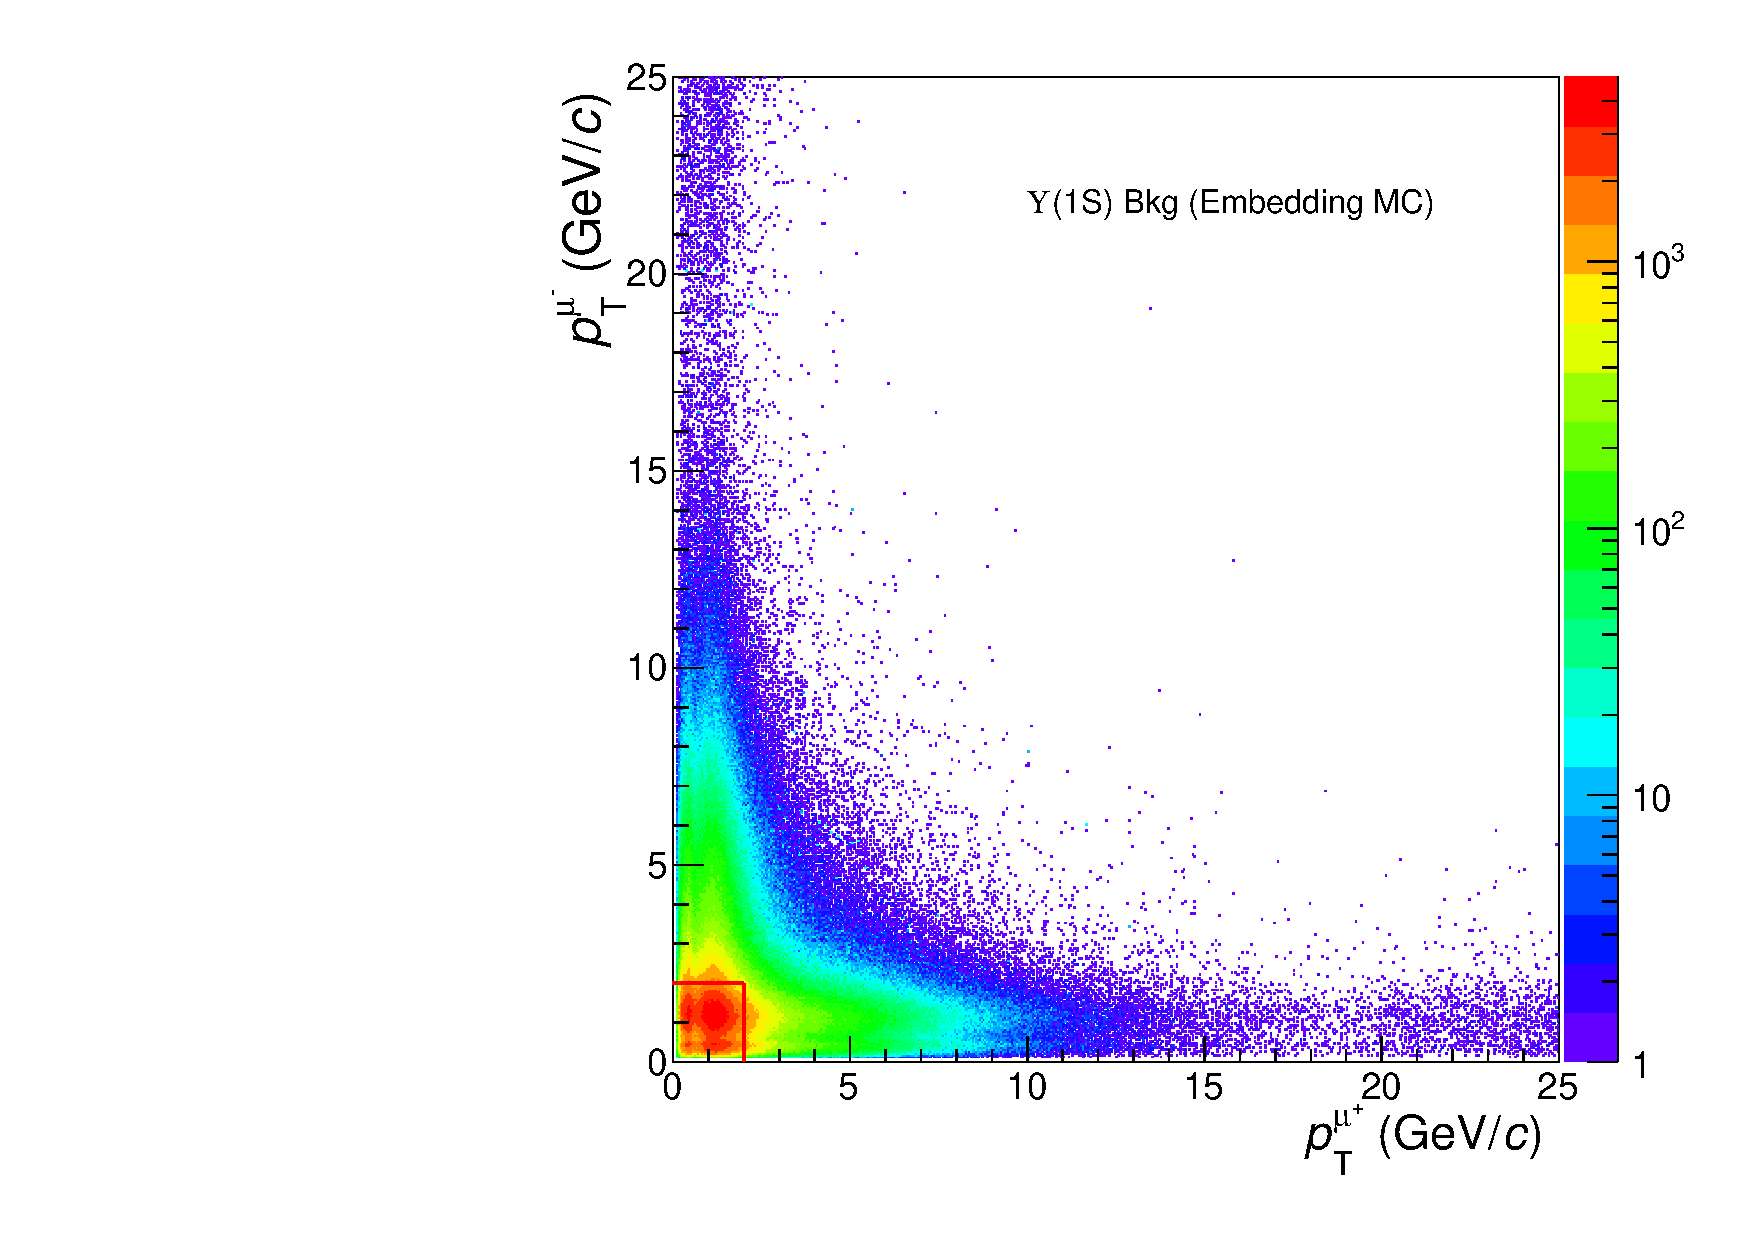
\includegraphics[width=0.45\linewidth]{Chapters/Analysis/Figs/background.pdf}
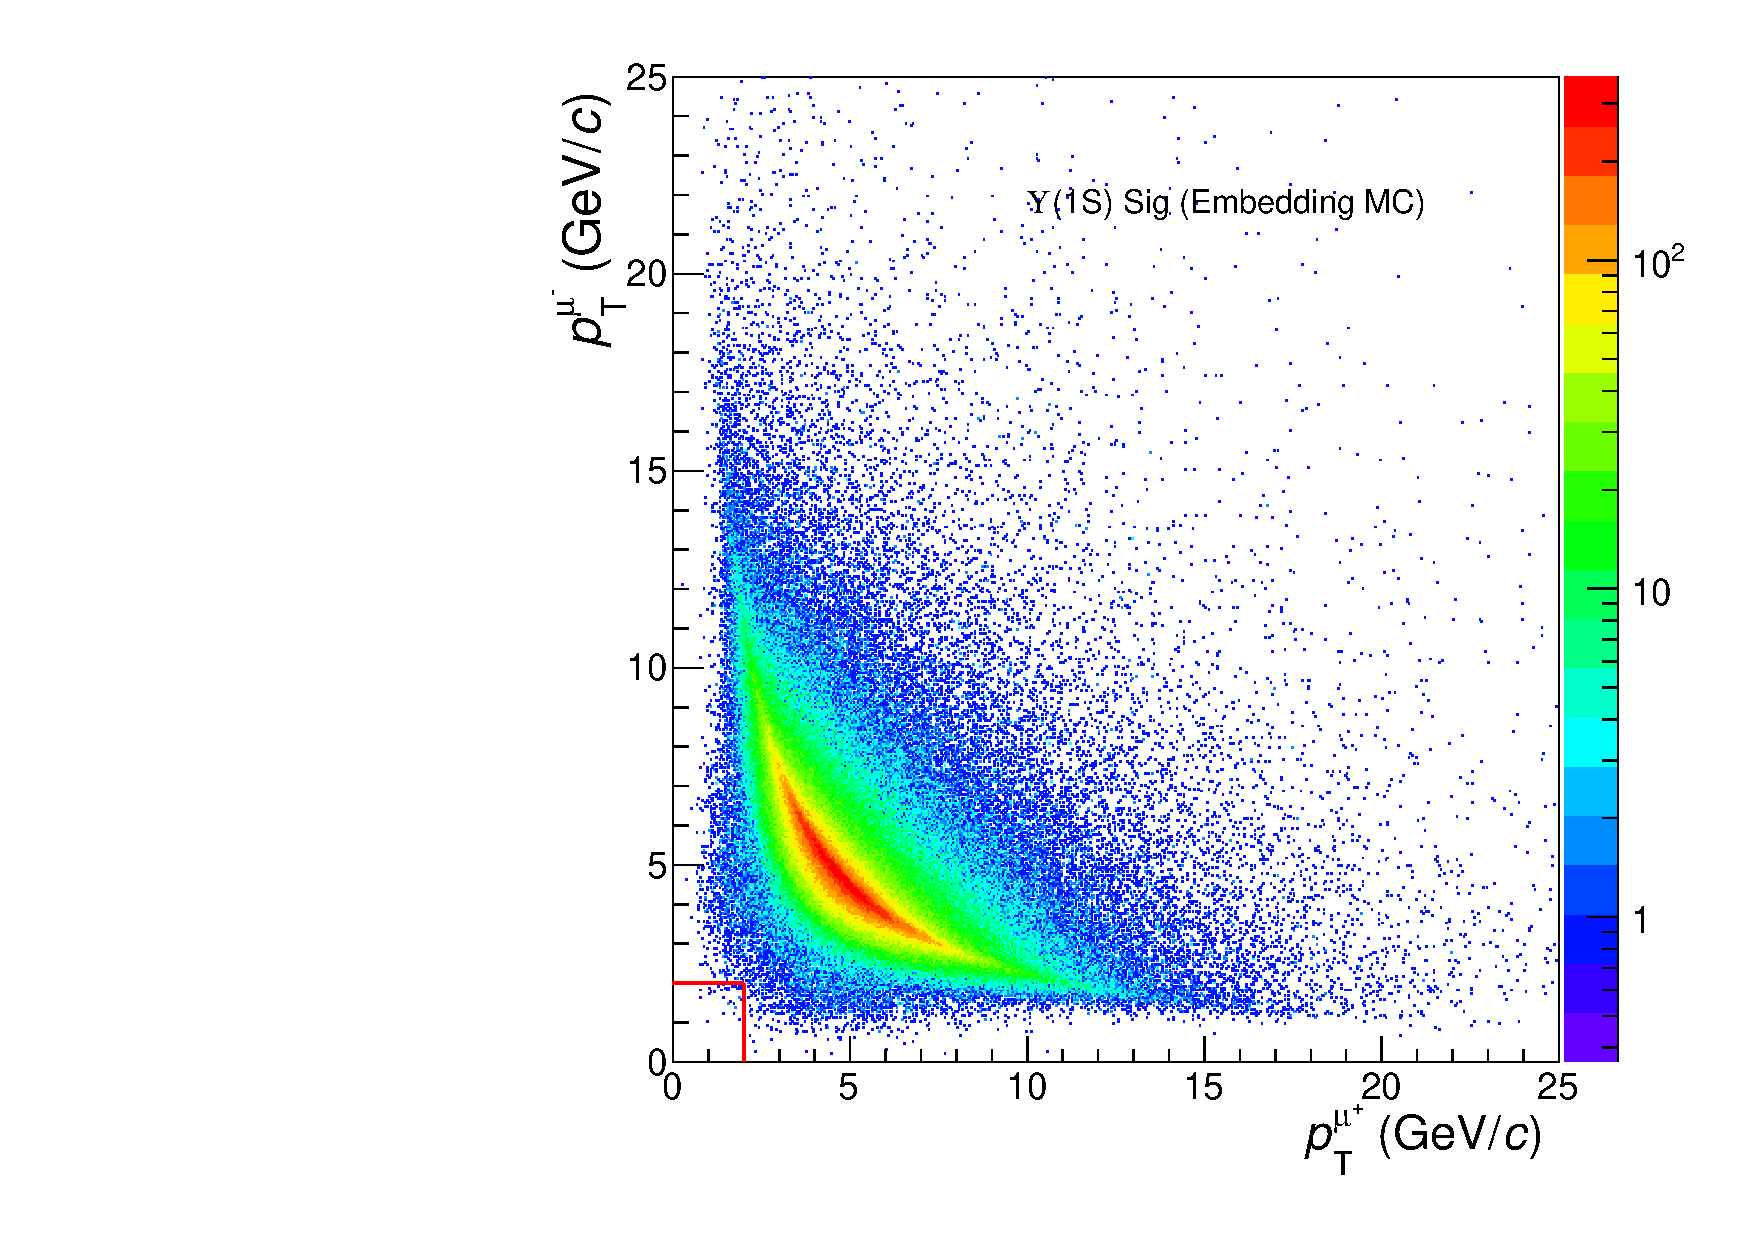
\includegraphics[width=0.45\linewidth]{Chapters/Analysis/Figs/signal.pdf}
\caption{Scatter plot of muon pair candidates' \pt~s for background candidates (left) and signal candidates (right). The cut at $p_{\rm{T}}=2 \rm{GeV}/c$ on both muons is represented as a red box.}
\label{fig:ptcut}
\end{center}
\end{figure}

The effect induced by that cut on \upsi yields was estimated by varying that cut by $\pm10$\%.
A $\pm2$\% maximum variation on the number of detected \upsi resonances, $N^{\Upsilon}$, was observed and included in the systematic uncertainties.

Various sources contribute to the systematic uncertainties of $A\times\epsilon$, such as input MC, the trigger efficiency, the track reconstruction efficiency and finally the matching efficiency between tracks in the muon tracking and triggering chambers. 

To evaluate the systematic uncertainty induced by the MC input shapes, various sets of simulations have been produced with different \upsi input \pt and $y$ distributions, obtained from empirical parameterizations and/or extrapolations of available data sets, such as ALICE data in \pbpb collisions at $\sqrt{s_{_{\rm NN}}}=5.02$~\rm{TeV}, $\sqrt{s_{_{\rm NN}}}=2.76$ \rm{TeV} and $pp$ collisions at $\sqrt{s}=5.02$~\rm{TeV} and CDF data in \pbpb at $\sqrt{s_{_{\rm NN}}}=4$~\rm{TeV}. 
The maximum relative difference of $A\times\epsilon$ obtained using the various input shapes is taken as the systematic uncertainty due to the MC input.
A summary of all the tests can be found in figure \ref{fig:MCsyst}.

\begin{figure}[!b]
\begin{center}
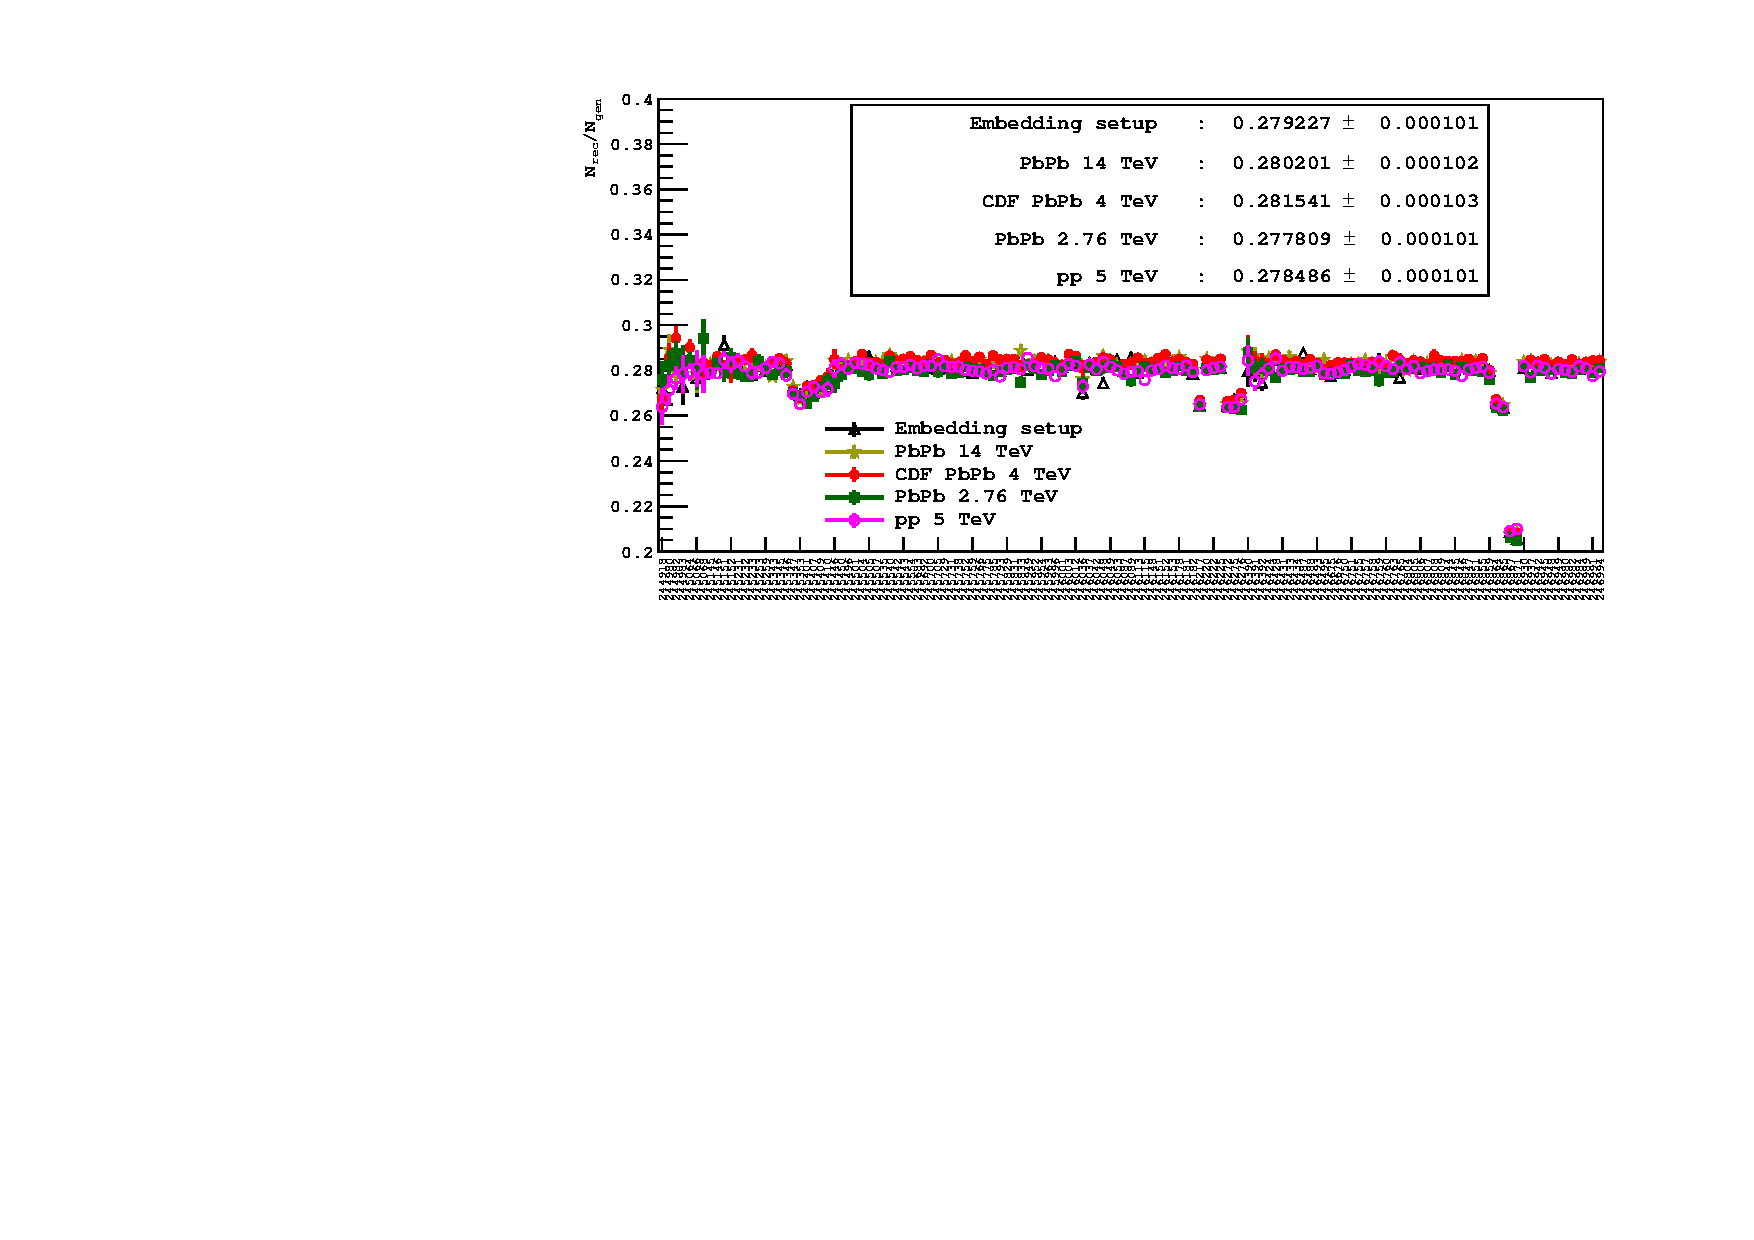
\includegraphics[width=\linewidth]{Chapters/Analysis/Figs/Axe/AxE_integrated.pdf}
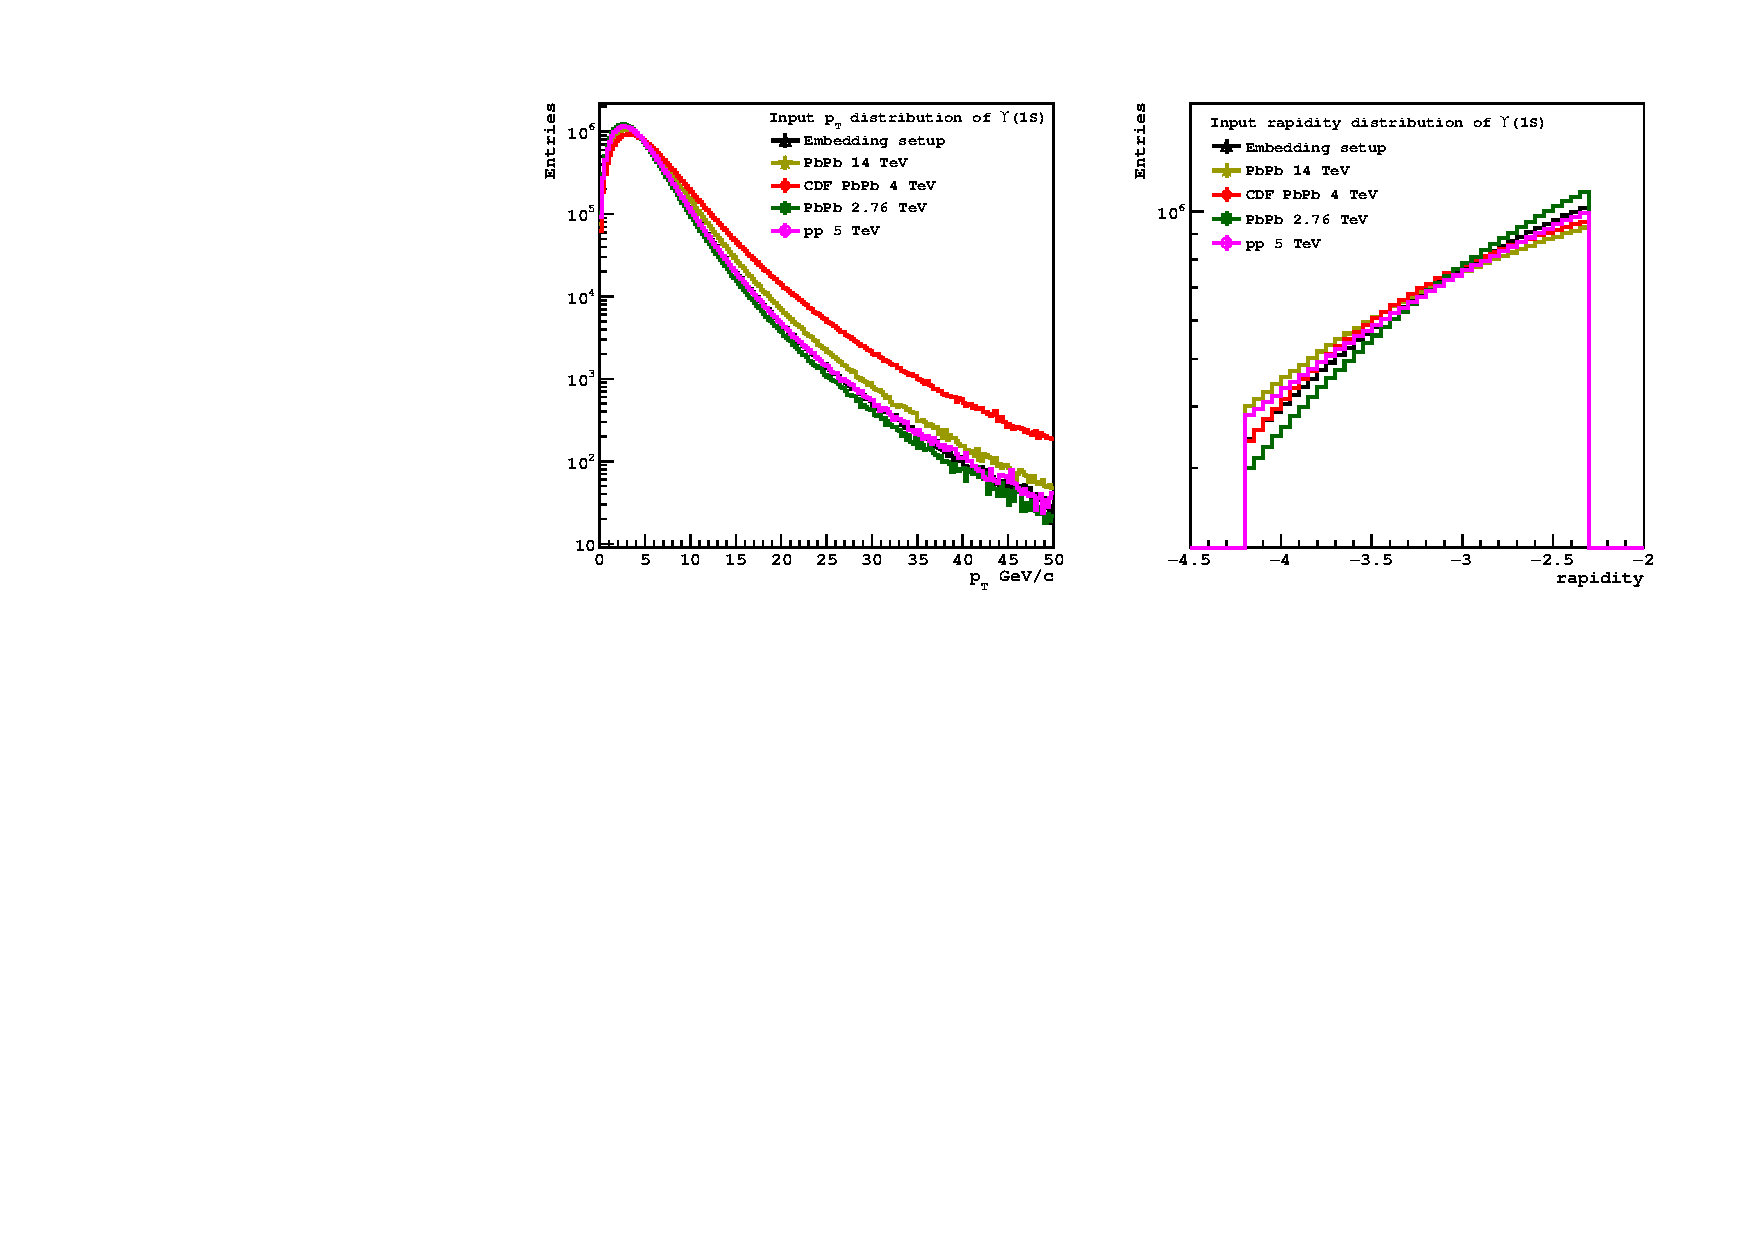
\includegraphics[width=0.9\linewidth]{Chapters/Analysis/Figs/input_pt_rap_dist.pdf}
\caption{Evolution of the $N_{rec}/N_{gen}$ ratio versus run number (top). Different colors refer to different input distributions for \upsis \pt and $y$ values, represented with the same color code in the bottom panel. Please note that the systematic study as a function of rapidity adopts an inverted convention for rapidity values, with respect to that adopted in this thesis, hence rapidity values are quoted as negative.}
\label{fig:MCsyst}
\end{center}
\end{figure}

In order to calculate the systematic uncertainty on the trigger efficiency, the trigger response function for single muons is evaluated using either MC or data.
The two response functions are then separately applied to simulations of a \upsi sample and the difference obtained for the \upsi reconstruction efficiency is taken as systematic uncertainty (see figure \ref{fig:trigsystRF}).

% In the same way as the modeled trigger response function in Monte Carlo may vary from the real situation, the muon trigger efficiency may follow the same path.
The Muon Trigger chamber efficiency is estimated from real data and gets plugged on the Monte Carlo simulations.
The uncertainty on the efficiency estimation leads to an uncertainty on the trigger efficiency.
In order to evaluate such uncertainty, two Monte Carlo productions have been performed.
The first simulation is performed using the efficiency value estimated using real data.
In the second simulation, the efficiency is artificially modified within its uncertainties.
The systematic uncertainty induced by this variation is then evaluated as the relative difference between the two.
The values obtained with the two chamber efficiency sets are reported in figure \ref{fig:trigsystAxe}.

\begin{figure}[!htb]
\begin{center}
% 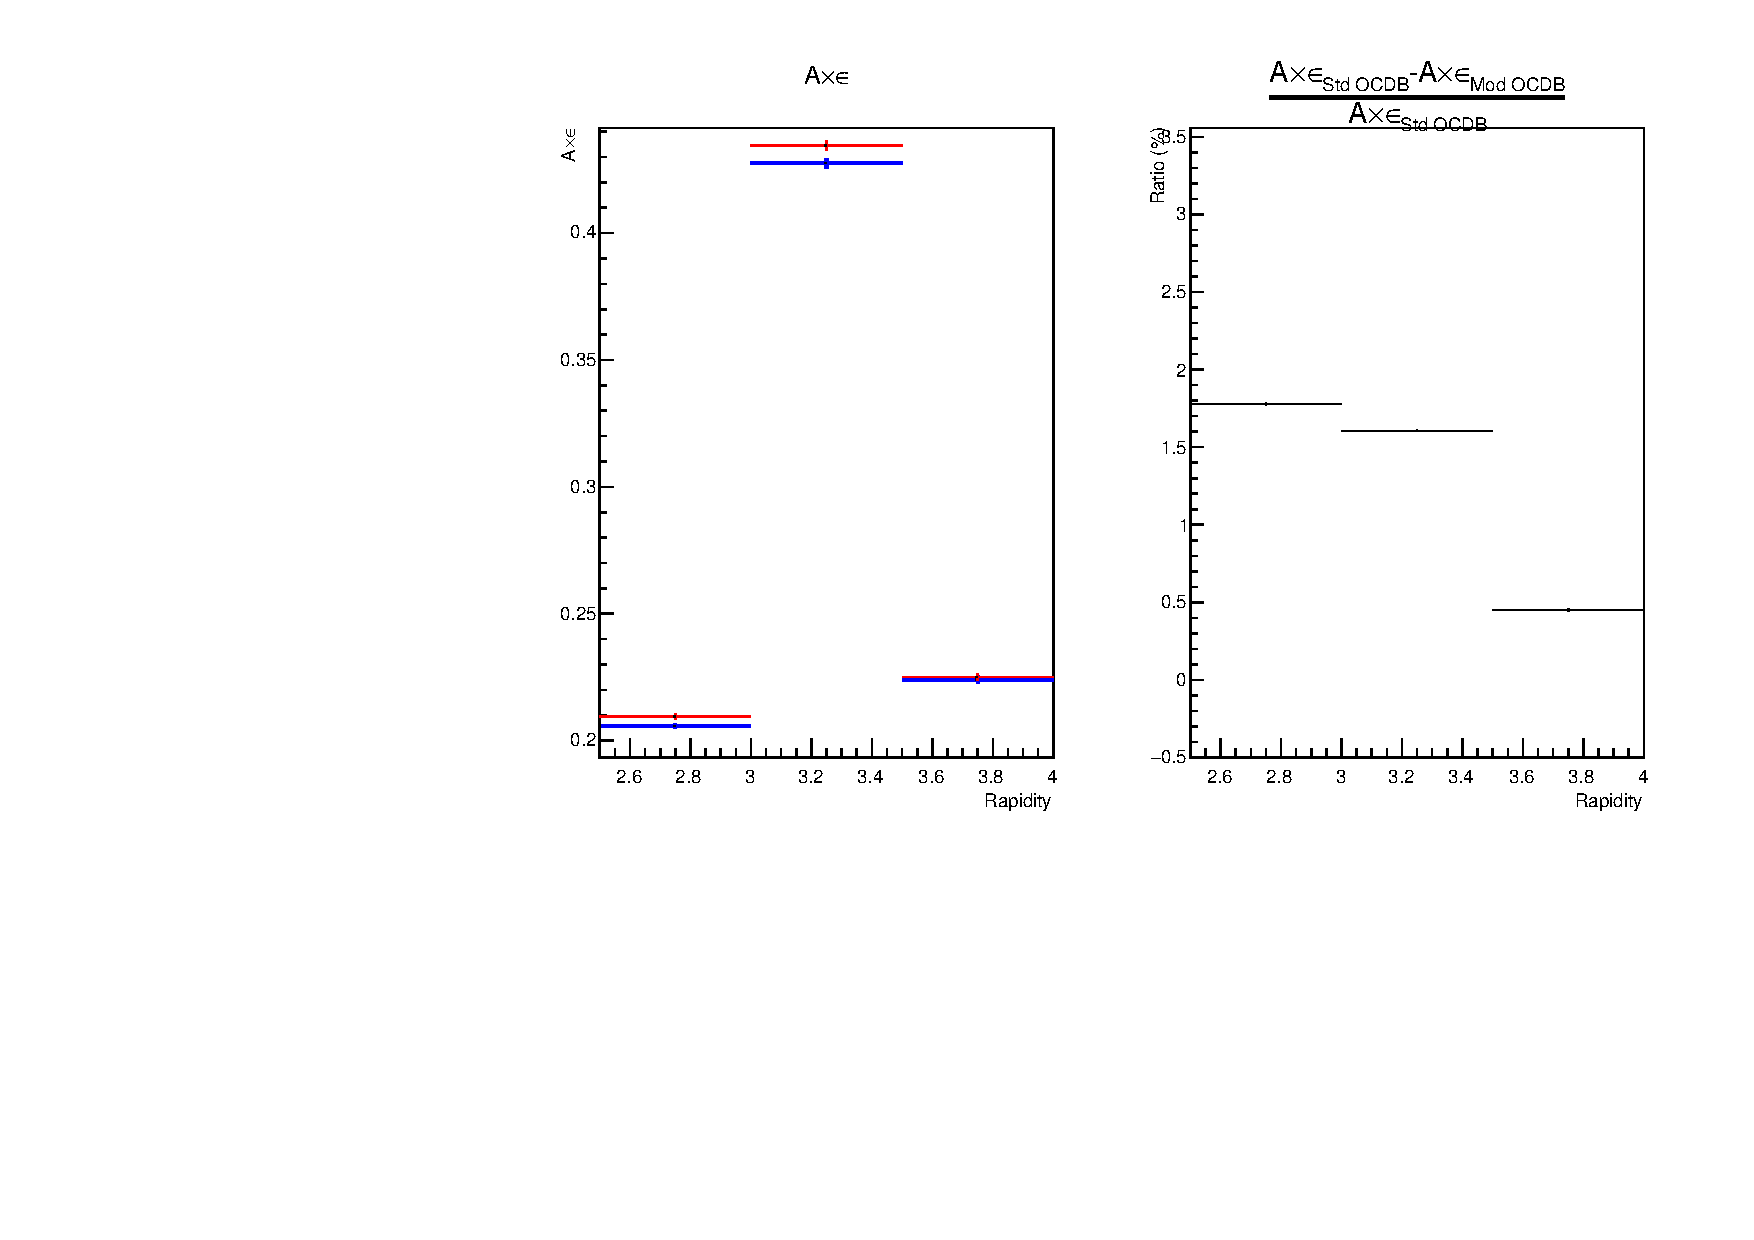
\includegraphics[width=0.45\linewidth]{Chapters/Analysis/Figs/AxEffSystError_NOCUT.pdf}
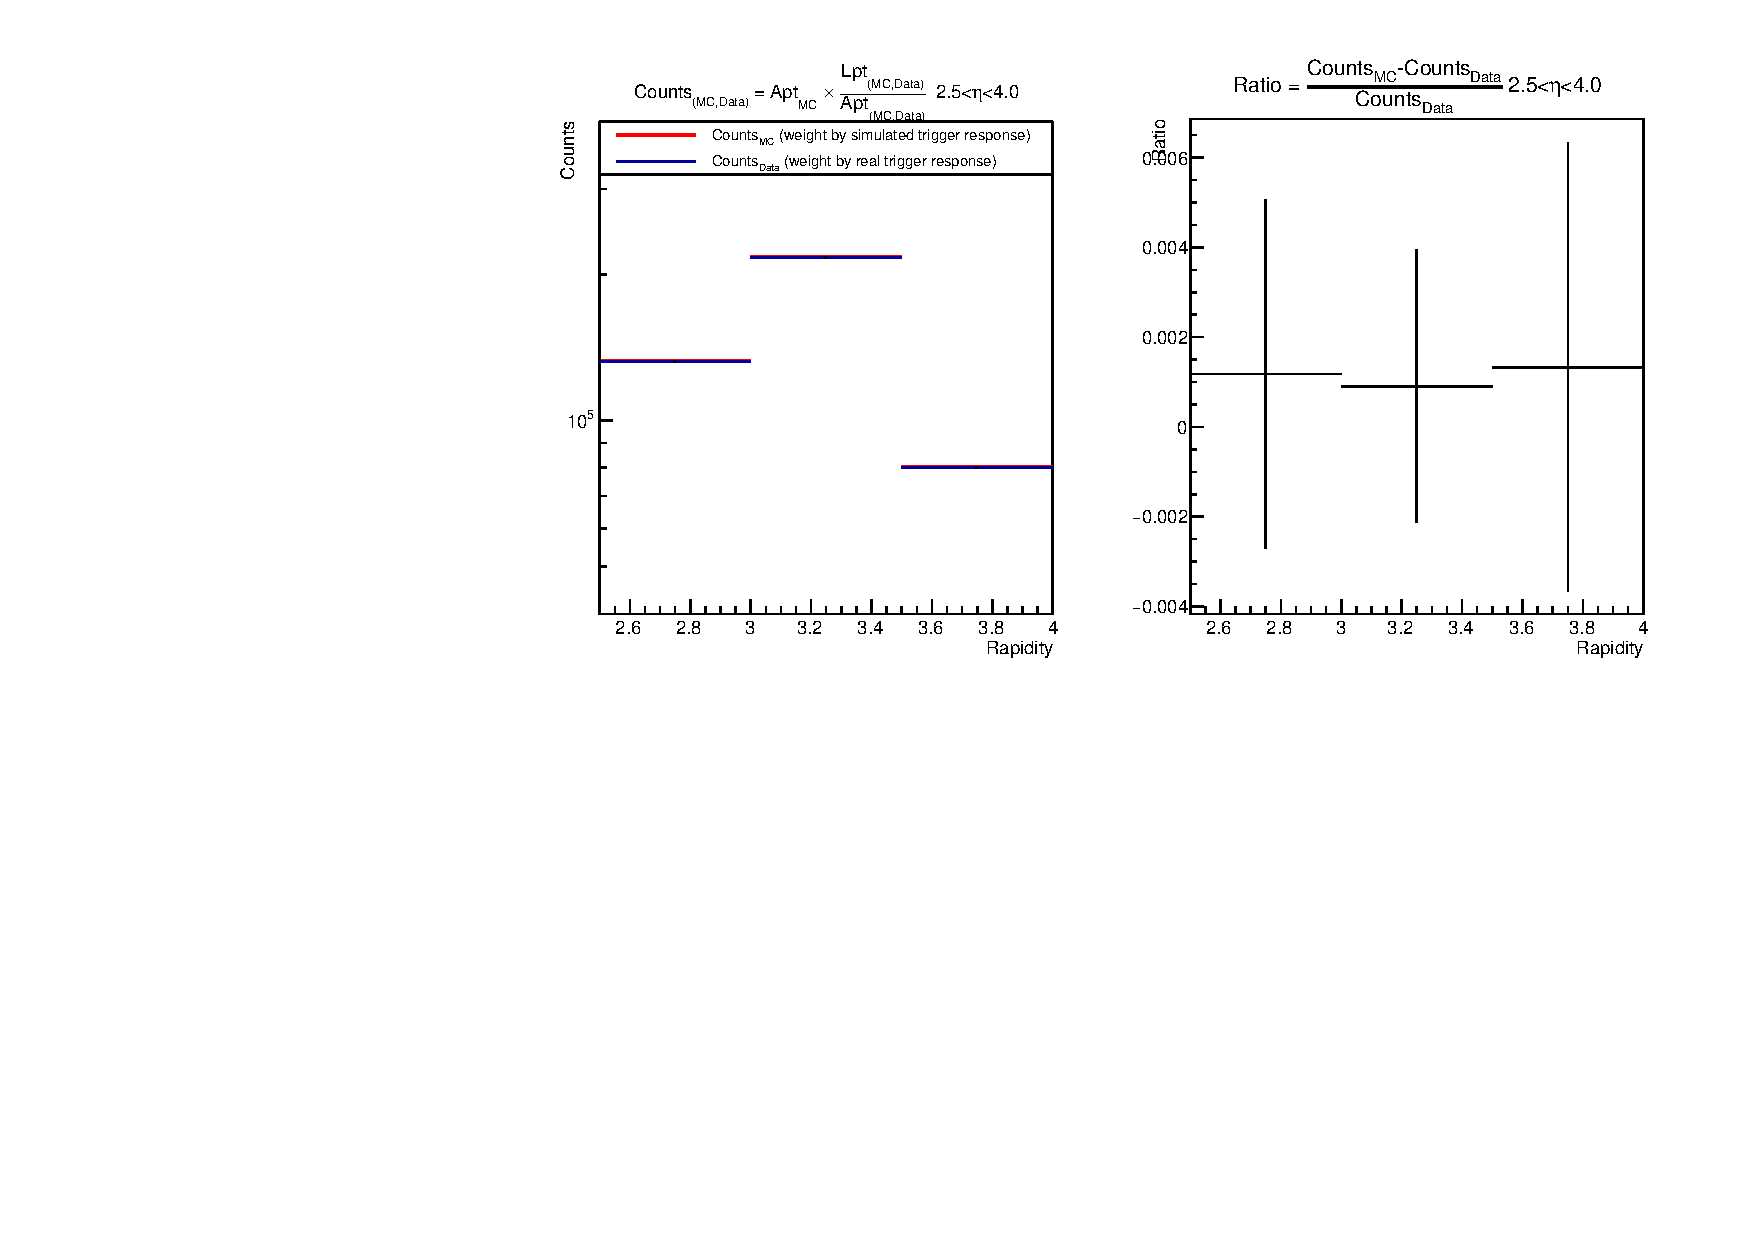
\includegraphics[width=0.9\linewidth]{Chapters/Analysis/Figs/ResponseFunctionSyst.pdf}
\caption{On left panel the muon trigger response function as a function of $y$ is shown. Trigger response is reweighted using Monte Carlo data (red) or real data (blue). Right panel shows the ratio of the two series as a function of $y$.}
\label{fig:trigsystRF}
\end{center}
\end{figure}

\begin{figure}[!htb]
\begin{center}
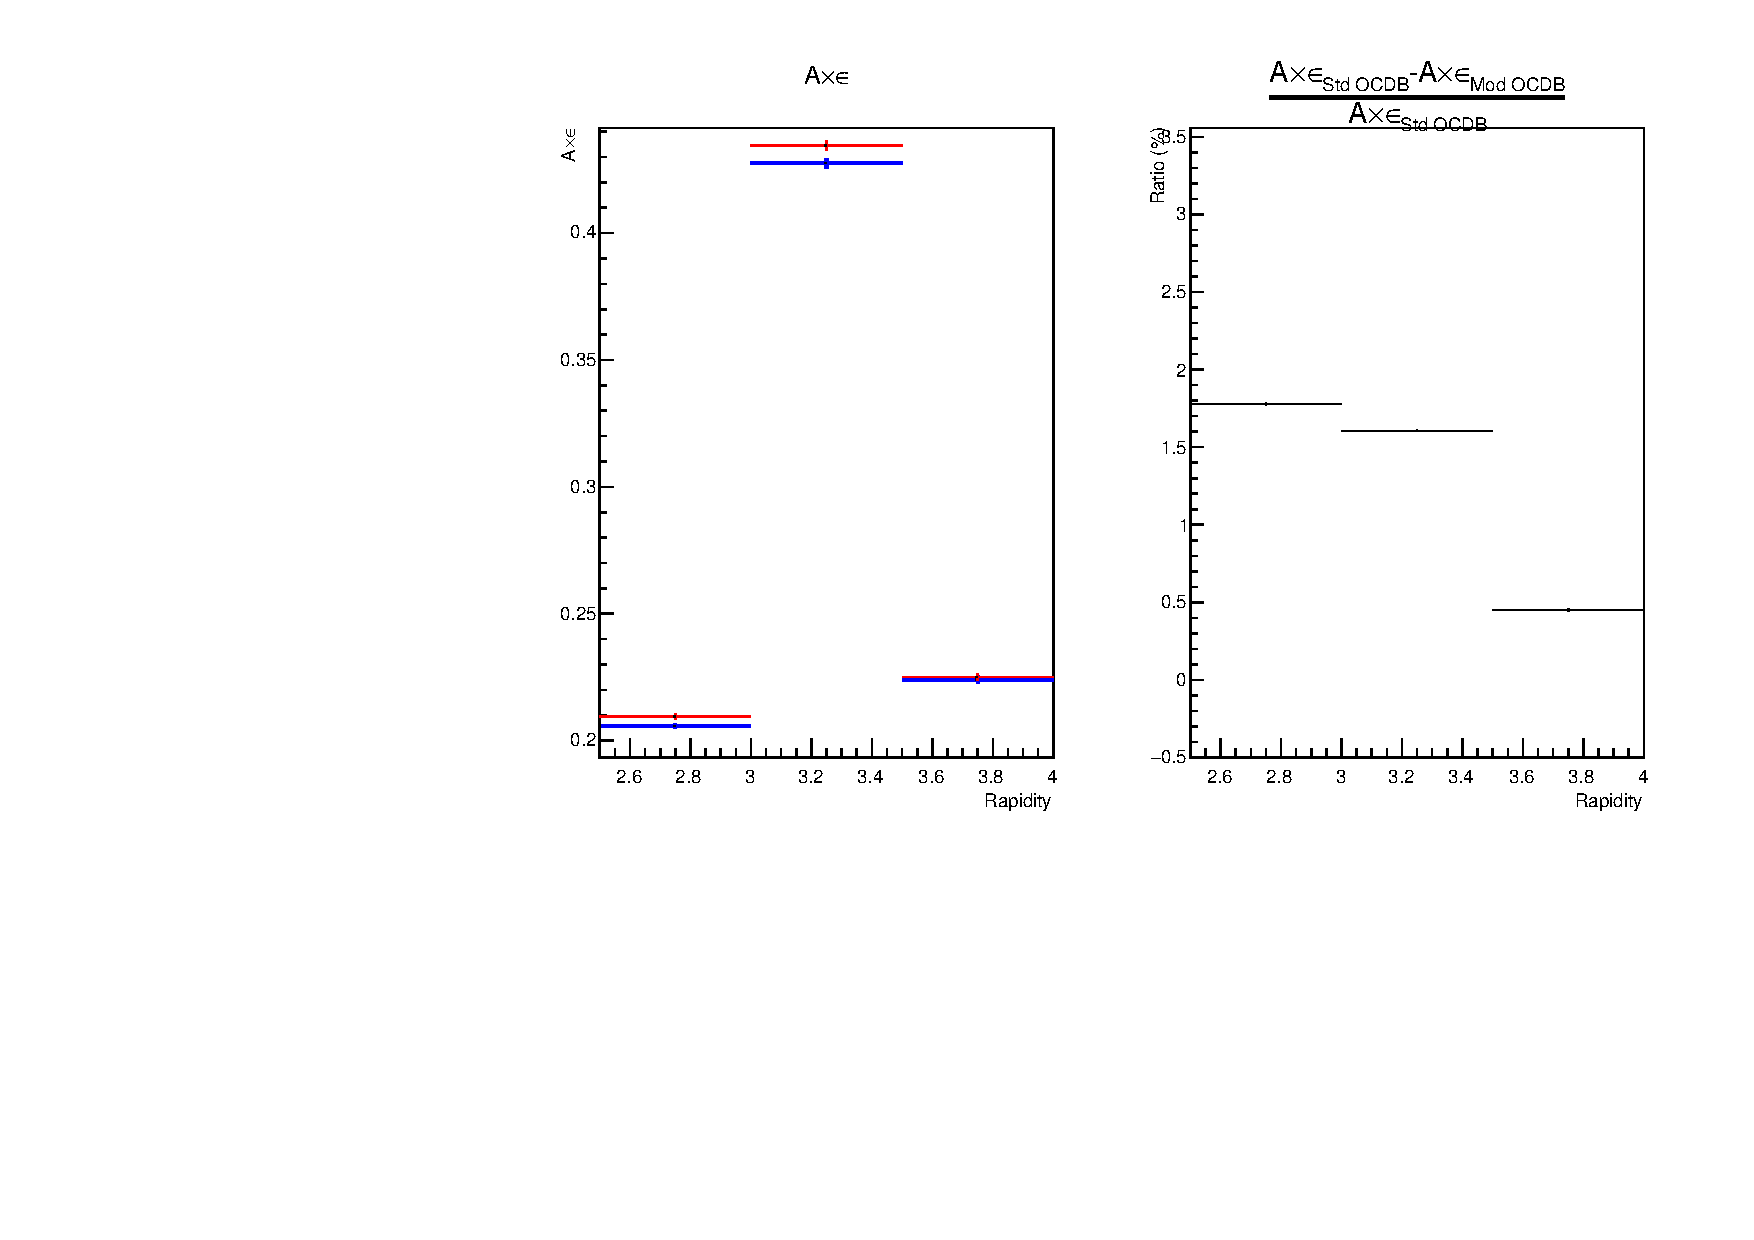
\includegraphics[width=0.9\linewidth]{Chapters/Analysis/Figs/AxEffSystError_NOCUT.pdf}
\caption{On left panel the muon trigger $A\times\epsilon$ as a function of $y$ is shown. Trigger efficiency is evaluated as the standard Monte Carlo set (red) or the real one (blue). Right panel shows the ratio of the two series as a function of $y$.}
\label{fig:trigsystAxe}
\end{center}
\end{figure}

The systematic uncertainty on the tracking efficiency is obtained starting from an evaluation of the single muon tracking efficiency in MC and data. 
This evaluation is performed via a procedure, detailed in ~\cite{Adam:2015isa}, based on the redundancy of the tracking chamber information.
The \upsi reconstruction efficiency is then obtained by combining the single muon efficiencies of the two systems, namely muon trigger and muon tracker.
The systematic uncertainty generated by the \upsi reconstruction efficiency is taken as the relative difference of the values obtained with the procedure based on MC and data.

The muon tracks for data analysis are chosen based on a selection on the $\chi^2$ of the matching between a track segment in the trigger system with the extrapolation of a track in the tracking chambers. 
The matching systematics is obtained by varying the $\chi^2$ selection cut in data and MC and comparing the effects on the track reconstruction efficiency~\cite{Adam:2016rdg}.

The systematic uncertainty on the centrality measurement is evaluated by varying by $\pm0.5\%$ the V0 signal amplitude corresponding to $90\%$ of the hadronic cross section in \pbpb collisions.
This choice is driven by the fact that the $90\%$ bin is used as anchor point to define the centrality classes.

The systematic uncertainty on the evaluation of $\sigma^{\rm pp}_{\Upsilon}$ is detailed in section \ref{sec:ppxsection}.

Finally, the systematic uncertainty evaluation of $F_{\rm{norm}}$ and $\langle T_{\rm{AA}}\rangle$ are described in~\cite{Adam:2016rdg} and~\cite{Abelev:2013qoq}, respectively.

The different systematic uncertainty sources on the $\raa$ calculation are summarized in Table~\ref{tab:syst}.
The correlated systematic uncertainties as a function of centrality, $y$ or $p_{\rm{t}}$ are indicated as type I. The uncorrelated ones as type II.
% In the table systematic uncertainties are correlated with the change of centrality, $\pt$ or $y$, are quoted as correlated (type I), otherwise they are treated as uncorrelated (type II).  

\begin{table}[!t]
\centering
\resizebox{1\textwidth}{!}{
\begin{tabular}{|c|c|c|c|c|c|}
\hline
\multirow{2}{*}{sources} & \multicolumn{4}{c|}{$\upsis$} & $\upsiss$ \\
\cline{2-5}
& Centrality & $y$ & $\pt$ & Integrated & Integrated \\
\hline
Signal extraction                               		& 4.3-6.1\%(II)                   	& 4.2-6.8\%(II)                  	& 5.2-8.7\%(II)                	& 4.1\%  	& 21.7\%\\
Muon \pt cut                               		& 0.3-2.4\%(II)                   	& 0.1-1.2\%(II)                  	& 0.1-2.4\%(II)                	& 0.7\%  	& 0.7\%\\
Input MC                                        		& 0.9\%(I)                       		& 0.6-2.6\%(II)                   & 1-1.4\%(II)                	& 0.9\%  	& 0.9\%\\
Tracker efficiency                             		& 3\%(I) and 0-1\%(II)      		& 1\%(I) and 3\%(II)		& 1\%(I) and 3\%(II)   	& 3\%  	& 3\%\\
Trigger efficiency                                       	& 3\%(I)                        		& 1.4-3.7\%(II)                   & 0.4-2.6\%(II)                 	& 3\%  	& 3\%\\
Matching efficiency                                     & 1\%(I)                        		& 1\%(II)                     	& 1\%(II)	                  	& 1\%  	& 1\%\\
%Centrality                                      		& 0.2-2.4\%(II)                     	& 0\%(I)                      	& 0\%(I)	                   	& 0\%  	& 0\%\\
Centrality                                      		& 0.2-2.4\%(II)                     	& -                      		& -	                   		& -  		& - \\
$F_{\rm{norm}}$                               		& 0.5\%(I)                        		& 0.5\%(I)                     	& 0.5\%(I)	                  	& 0.5\%  	& 0.5\%\\
$\langle T_{\rm{AA}}\rangle$                  	& 3.1-5.3\%(II)                      	& 3.2\%(I)                     	& 3.2\%(I)	                   	& 3.2\% 	& 3.2\%\\
${\rm BR}_{\Upsilon \rightarrow \mu^{+} \mu^{-}} \cdot \sigma^{\rm pp}_{\Upsilon}$                 	& 6.3\%(I)		                        	& 6.6-11.3\%(II)                 	& 5.5-11.5\%(II)		        	& 6.3\% 	& 7.5\%\\
\hline
\end{tabular}
}
\caption{\label{tab:syst}Summary of the systematic uncertainties for $\raa$ calculation. Type I (II) refers to correlated (uncorrelated) systematic uncertainties.}
\end{table}

%%%%%%%%%%%%%%%%%%
%%%%% DONE! %%%%%%
%%%%%%%%%%%%%%%%%%

%%%%%%%%%%%%%%%%%%%%%%%%%%%%%%%%%%%%%%%%%%%%%%%%
\section{Results}\label{section:results}

The nuclear modification factors for  inclusive $\upsis$ and $\upsiss$ production in \pbpb collisions at $\snn=5.02$ \rm{TeV} with $p_{\rm T} < 15$ GeV/$c$, $2.5 < y < 4$ and the 0--90\% centrality class are $R_{\rm{AA}}^{\Upsilon(\rm1S)}=0.37\pm0.02\text{(stat)}\pm0.03\text{(syst)}$  and $R_{\rm{AA}}^{\Upsilon(\rm2S)}=0.10\pm{0.04}\text{(stat)}\pm{0.02}\text{(syst)}$, respectively.
The quantities entering the \raa for the \upsiss have been determined exactly in the same ways as those for the \upsis.
The measurements show a strong suppression for both bottomonium states.

The value of the systematic uncertainties affecting the $R_{\rm{AA}}$ is comparable to those of the statistical ones.
To reduce the contribution of systematic uncertainties the ratio of the two $R_{\rm{AA}}$ can be computed.
% Since the decay kinematics of \upsis and \upsiss states are very similar, most of the systematic uncertainty sources entering the ratio cancel out.
However the dominant contributions to the systematic uncertainties, namely those related to signal extraction and the $pp$ cross section, are not simplified by the computation of the ratio.
The integrated ratio $R_{\rm{AA}}^{\Upsilon(\rm2S)}/R_{\rm{AA}}^{\Upsilon(\rm1S)}$ is $0.28\pm0.12\text{(stat)}\pm0.06\text{(syst)}$. 
An indication of a stronger suppression for \upsiss around $2.5\sigma$ is present.

A comparison between \upsis nuclear modification factor values at different energies might highlight a suppression dependence on the center of mass energy of the colliding system.
The ratio between the \upsis $\raa$ at $\snn=5.02$ \rm{TeV} and $2.76$ \rm{TeV} is $1.23\pm0.21\text{(stat)}\pm0.19\text{(syst)}$. 
The sources of systematic uncertainties entering the calculation of the ratio are considered uncorrelated, except for the \taa component, whose uncertainty cancels out. 
The ratio is compatible with unity within uncertainties, hence no energy dependence is observed within the present uncertainties.

%The centrality, $p_{\rm T}$- and $y$-dependences of the $\upsis \raa$ at forward rapidity at $\snn=5.02$ \rm{TeV} are shown in Fig.\ref{fig:raa_data} together with the published results by CMS at mid-rapidity at the same center-of-mass energy \cite{CMS:2017ucd}. 
The centrality, $p_{\rm T}$ and $y$-dependences of the $\upsis$ $\raa$ at forward rapidity at $\snn=5.02$ \rm{TeV} are shown in figure \ref{fig:raa_data}. 
A decrease of $\raa$ with increasing centrality is observed down to $R_{\rm{AA}}^{\Upsilon(\rm1S)}=0.33\pm0.03\text{(stat)}\pm0.03\text{(syst)}$  for the 0--10\% most central collisions.
The $p_{\rm T}$-dependence is observed to be compatible within uncertainties with a flat behaviour up to $p_{\rm T}=15$ GeV/$c$.
The $y$-dependence shows a $\raa$ compatible within uncertainties with a flat distribution, as already observed in the measurements at $\snn=2.76$ \rm{TeV} \cite{Abelev:2014nua}.
However, since the uncertainties are large especially at low pt, further dara are needed in order to have a stronger conclusion on the rapidity dependence of the $\raa$.

\begin{figure}[!t]
\begin{center}
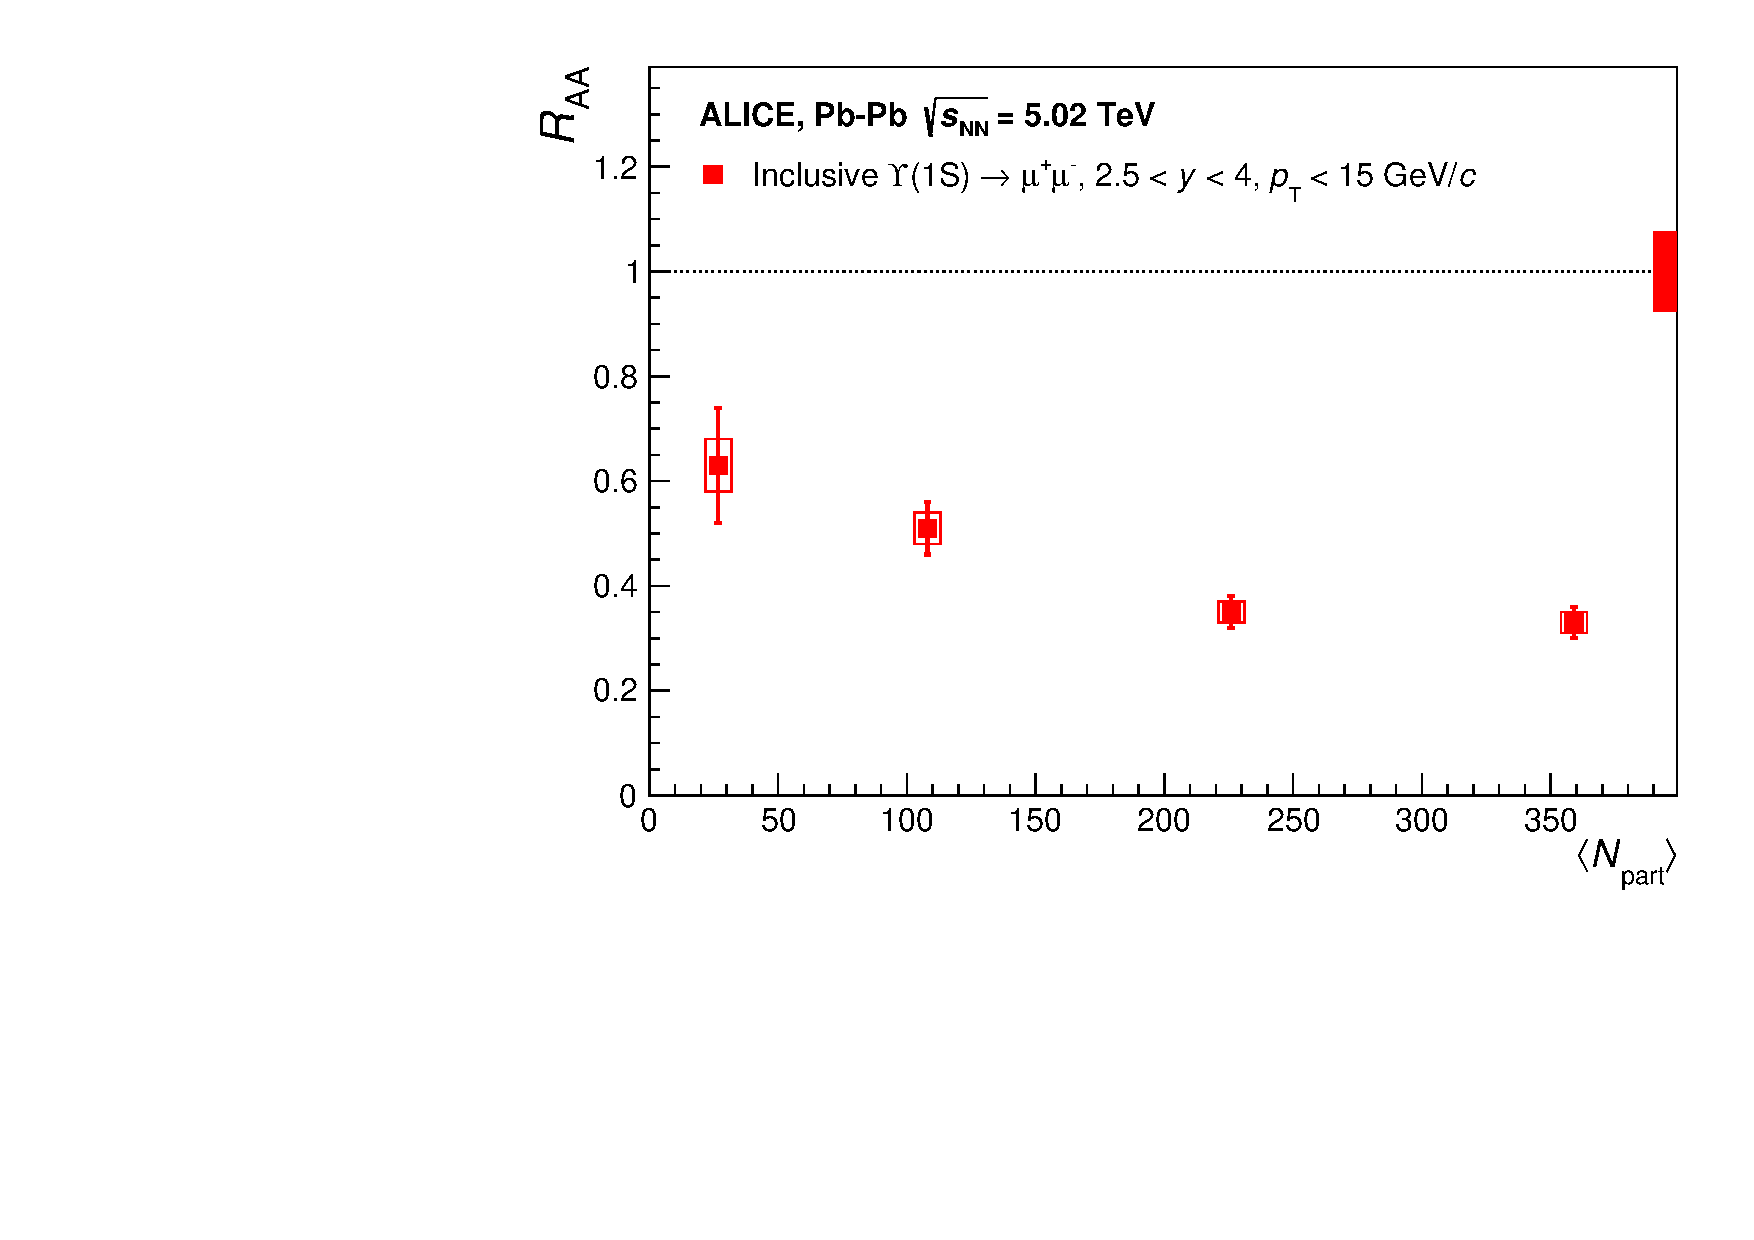
\includegraphics[width=0.9\linewidth]{Chapters/Analysis/Figs/RAA_Cent_ALICE2015.pdf} \\ 
%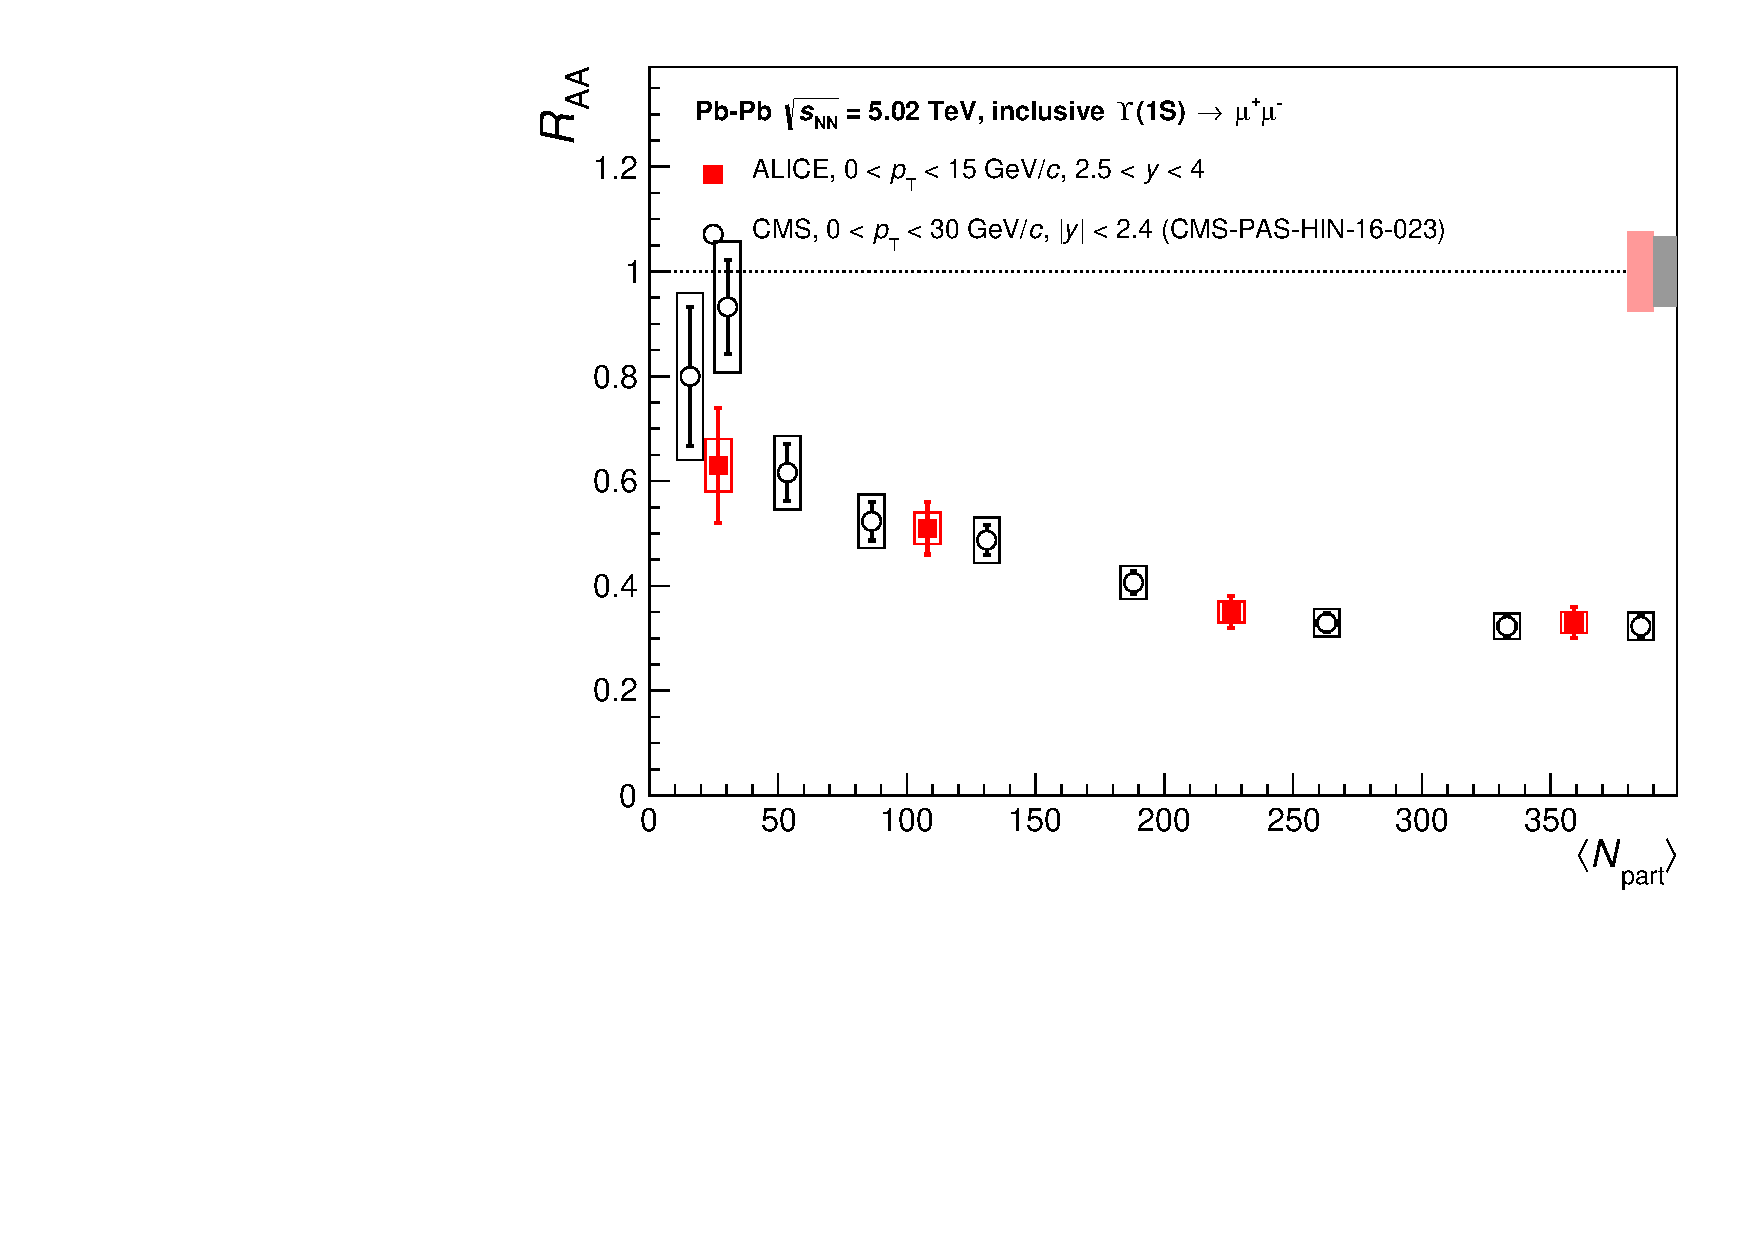
\includegraphics[width=0.5\linewidth]{RAA_Cent_ALICE2015vsCMS2015.pdf} \\ 
\end{center}
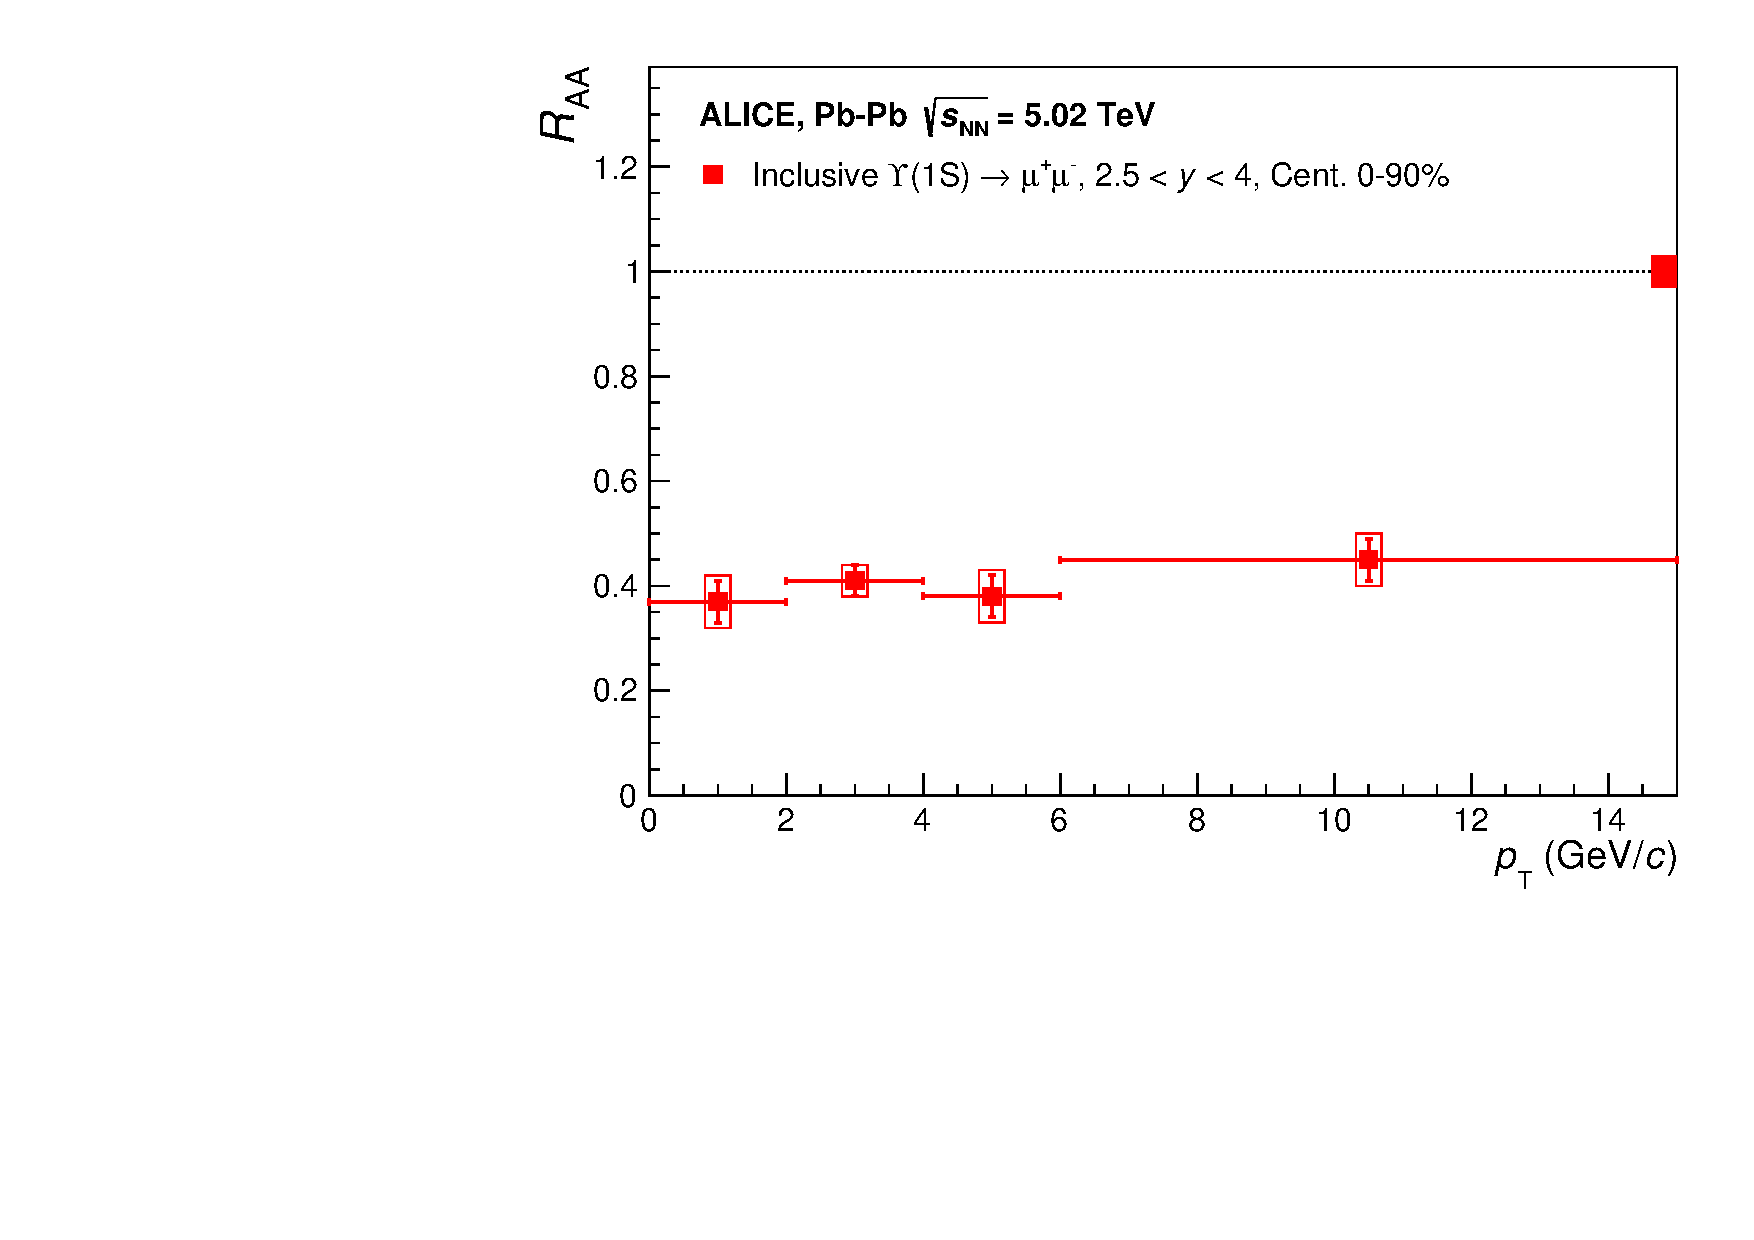
\includegraphics[width=0.5\linewidth]{Chapters/Analysis/Figs/RAA_Pt_ALICE2015.pdf}
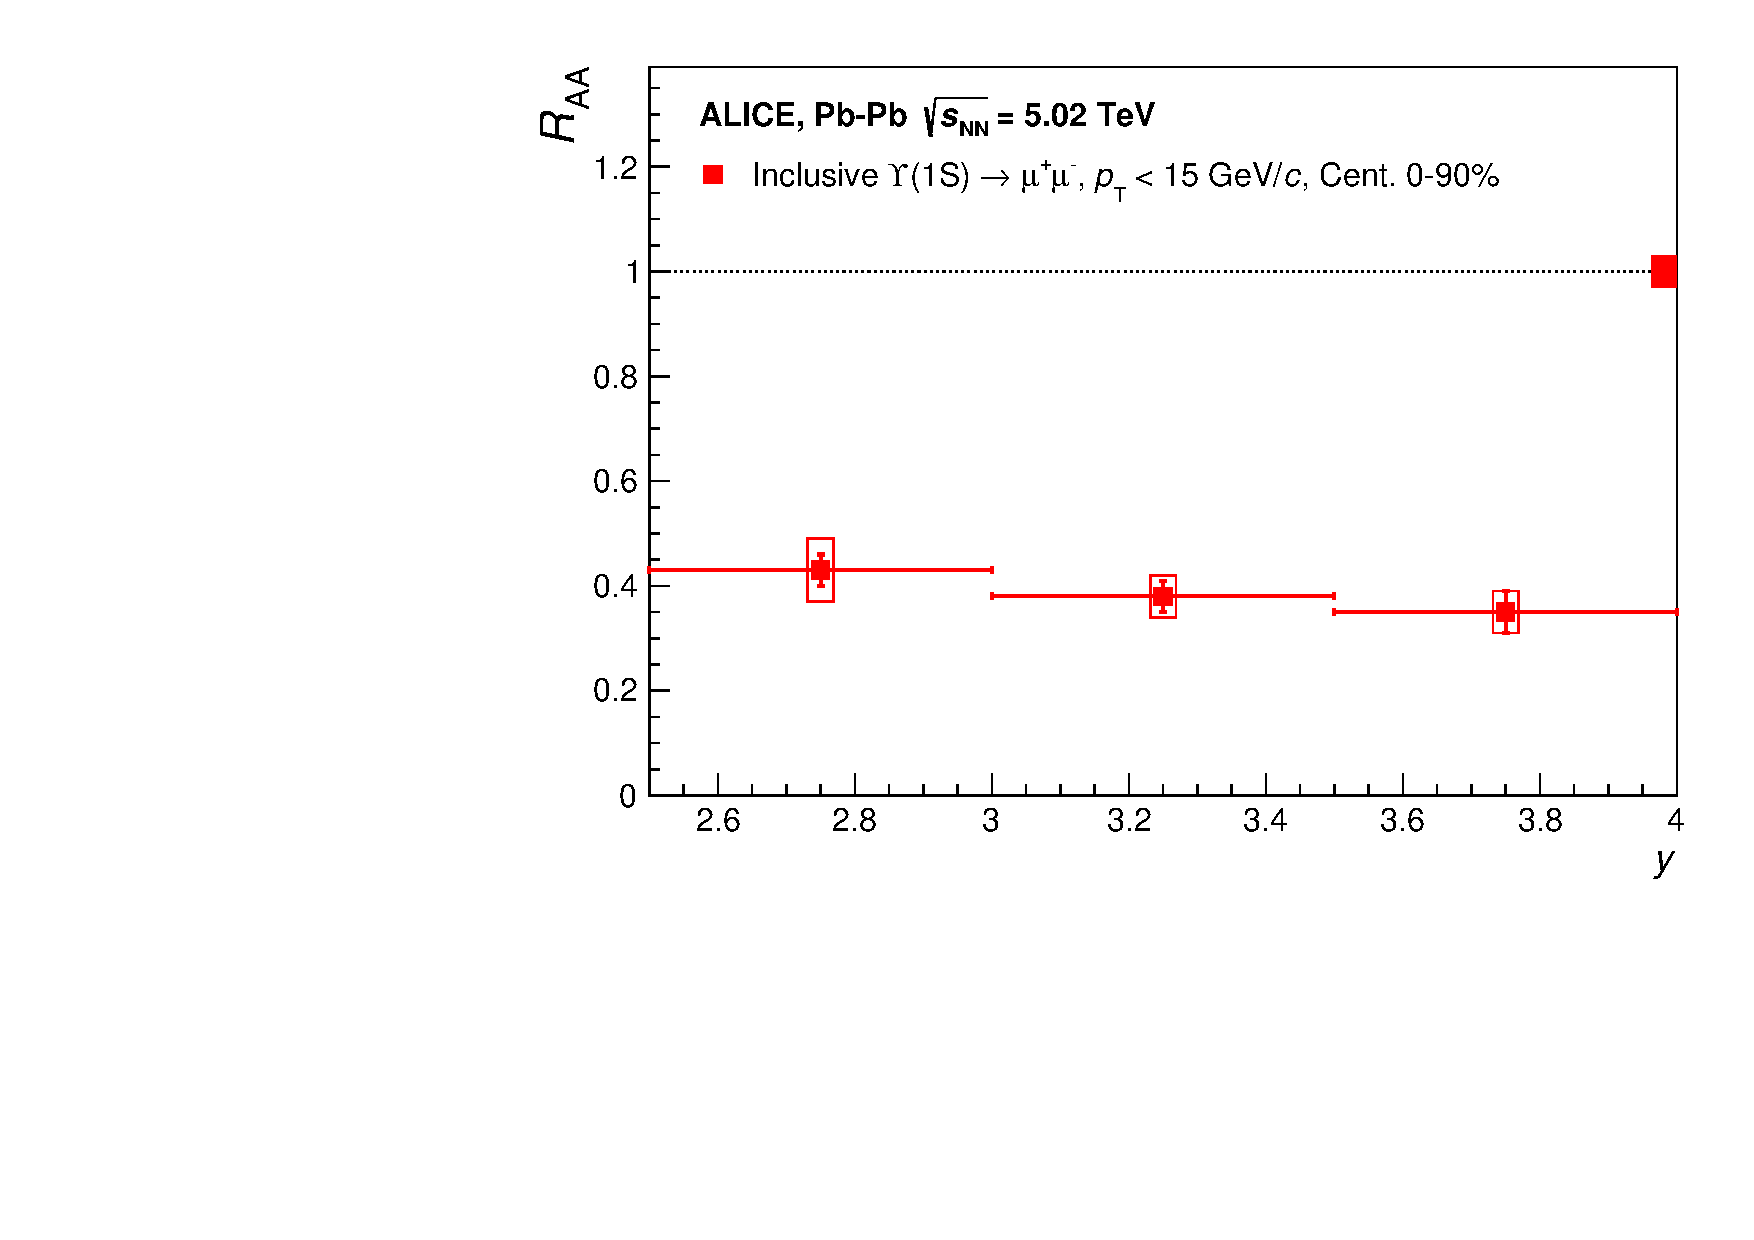
\includegraphics[width=0.5\linewidth]{Chapters/Analysis/Figs/RAA_Y_ALICE2015.pdf}
%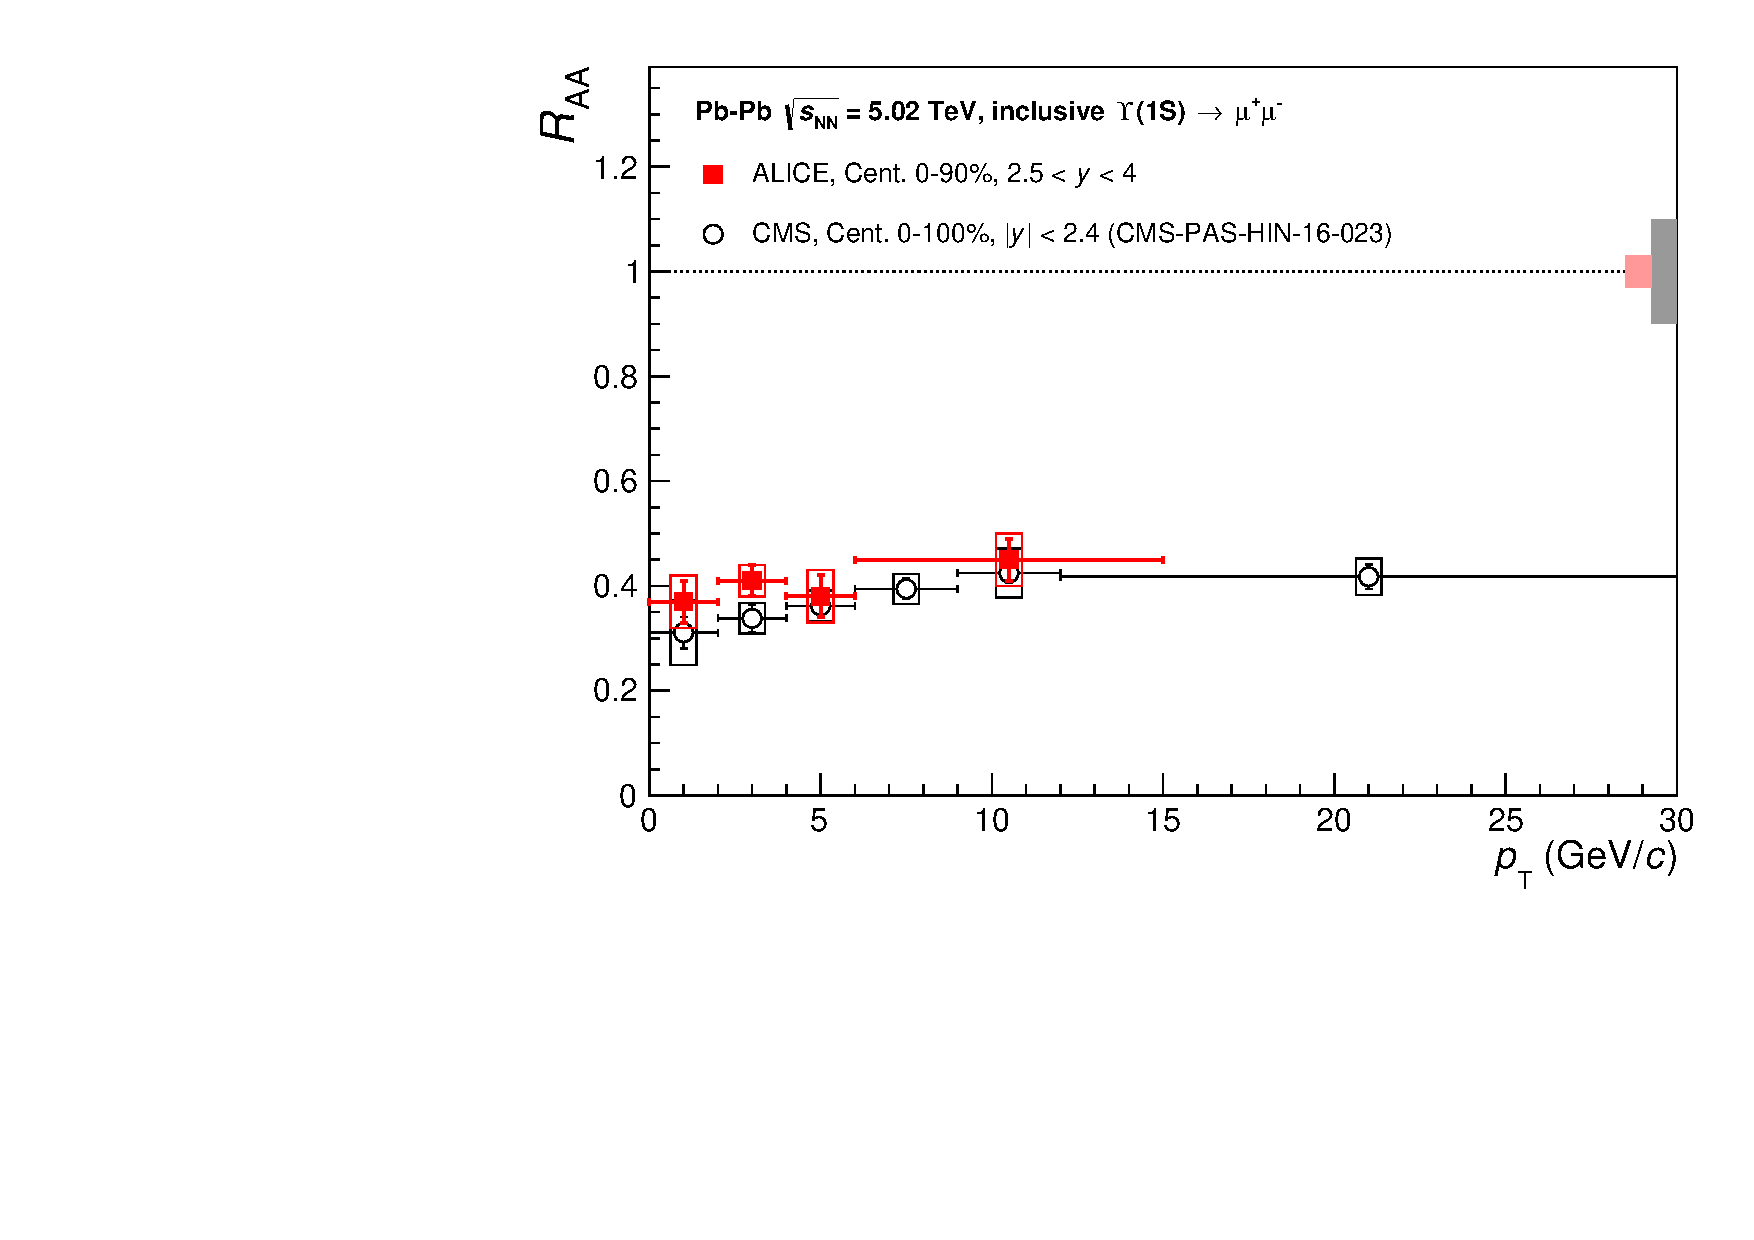
\includegraphics[width=0.5\linewidth]{RAA_Pt_ALICE2015vsCMS2015.pdf}
%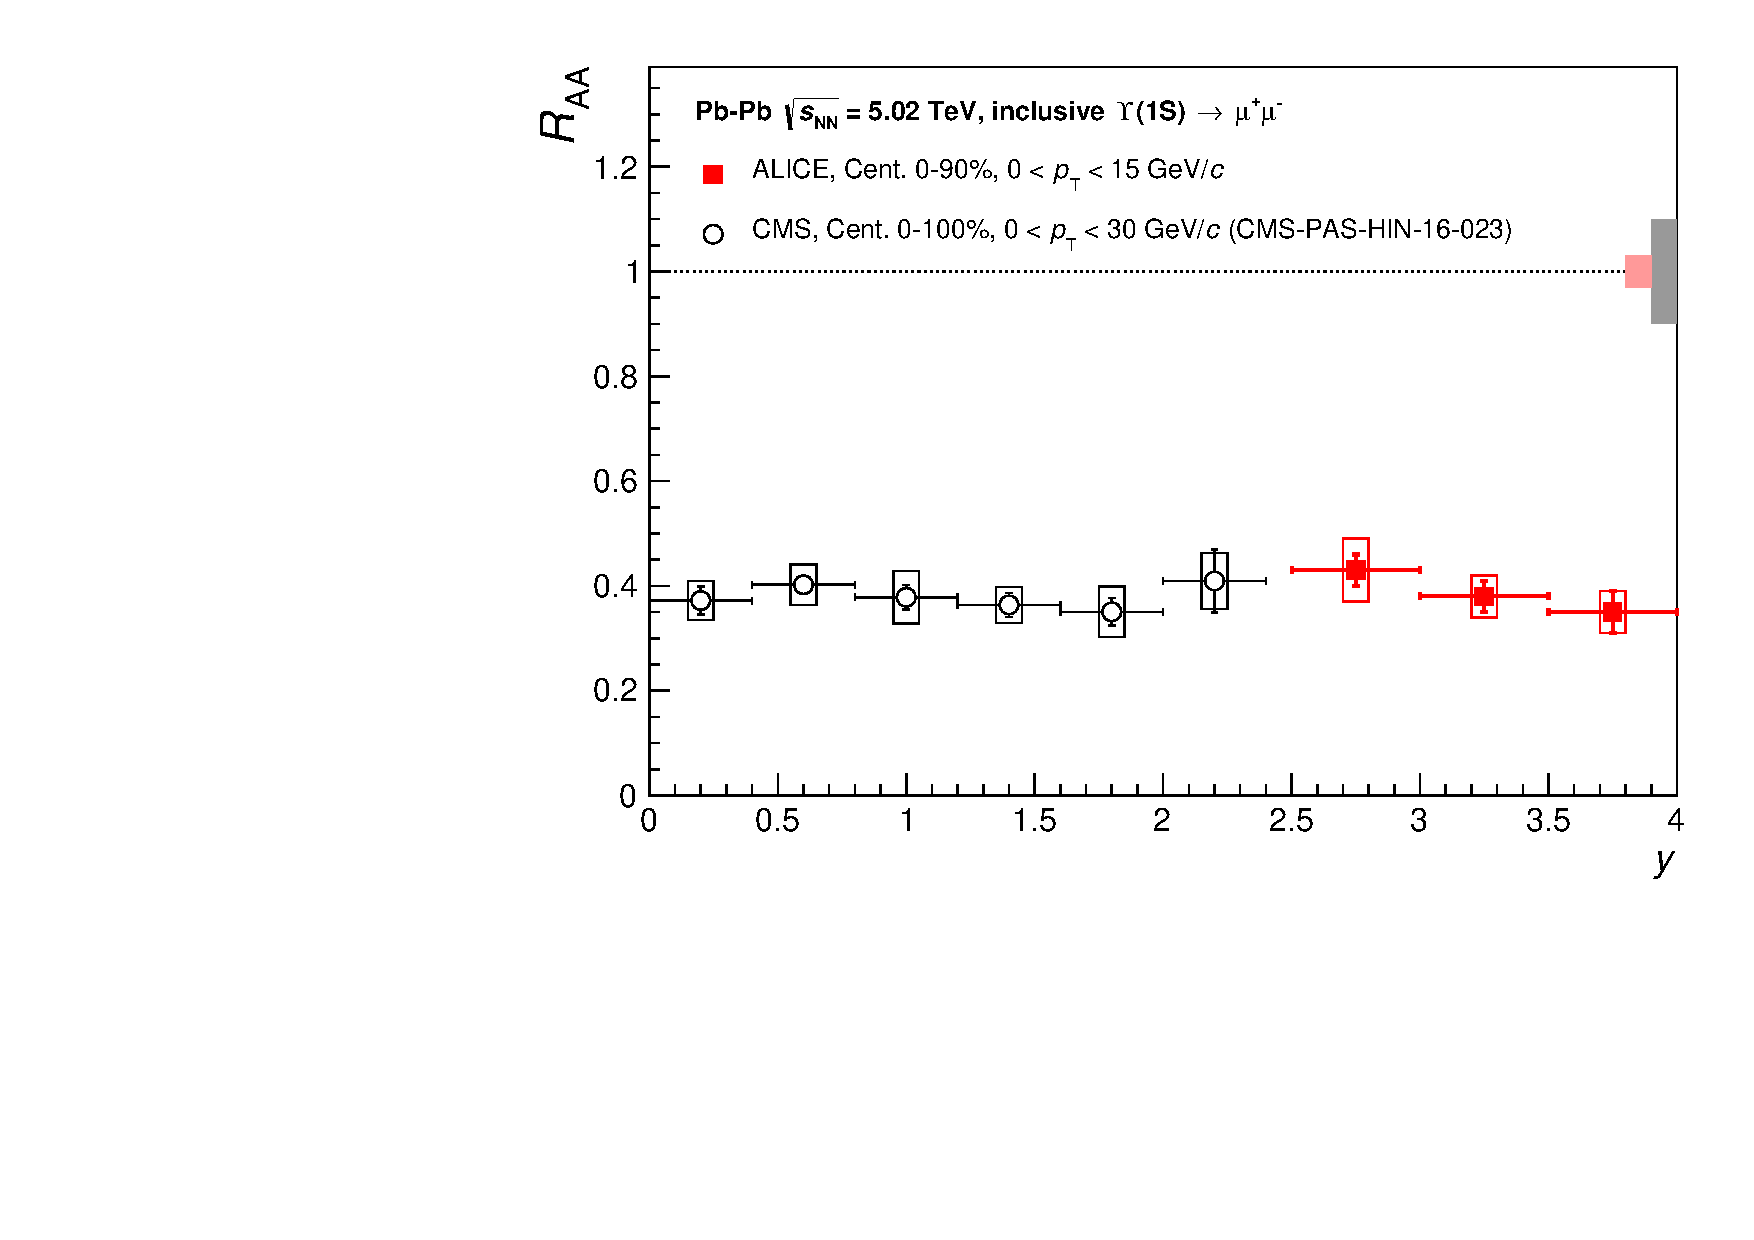
\includegraphics[width=0.5\linewidth]{RAA_Y_ALICE2015vsCMS2015.pdf}
\caption{Inclusive $\upsis$ $\raa$ as a function of centrality (top), $\pt$ (left) and $y$ (right) at forward rapidity at $\snn=5.02$ \rm{TeV}. The vertical error bars and the boxes represent the statistical and uncorrelated systematic uncertainties, respectively. The relative correlated uncertainty is shown as boxes at unity.}
%\caption{Inclusive $\upsis$ $\raa$ as a function of centrality (top), $\pt$ (left) and $y$ (right) at forward rapidity (full red squares) at $\snn=5.02$ \rm{TeV} together with the CMS results at mid-rapidity (open black circles). The vertical error bars and the boxes represent the statistical and uncorrelated systematic uncertainties, respectively. The relative correlated uncertainties are shown as a box at unity.}
\label{fig:raa_data}
\end{figure}

The inclusive $\upsis$ $\raa$ measurements are compared to several theoretical predictions in Fig. \ref{fig:raa_models}.
The set of models used for comparison is composed by two transport models (TM1 and TM2)\cite{Du:2017qkv,Zhou:2014hwa} and one hydro-dynamical model \cite{Krouppa:2017jlg}.
While transport models follow the propagation of the free quarks in the medium, the hydro-dynamical models approach the QGP as a macro state.
Transport models use a rate-equation approach which accounts for both suppression and (re)generatio mechanisms in the QGP.
In hydro-dynamical models, the macro state "decays" in micro states ($e.g$ quarkonium states, open heavy flavor hadrons) at the freeze-out.

In the model quoted as TM1 \cite{Du:2017qkv}, the evolution of the thermal medium is based on a thermal-fireball expansion.
The feed-down contribution is taken into account based on measurements from ALICE and LHCb \cite{Abelev:2014qha,Aaij:2014caa,Aaij:2014hla}.
TM1 predictions are shown as bands, obtained varying the magnitude of nuclear shadowing effects, as described in ~\cite{Tuchin:2010pv}. 
The upper limit shown in Fig.~\ref{fig:raa_models} corresponds to the extreme case of the absence of shadowing while the lower limit reflects a reduction of $30\%$ due to shadowing.

TM2 \cite{Zhou:2014hwa} uses a 2+1 dimensional version of ideal hydrodynamic equations.
The uncertainties on these predictions are given by the spread caused by two sets of feed-down fractions to \upsis ground state:
\begin{itemize}
\item $27\%$ from $\chi_{\rm b}$; $11\%$ from $\Upsilon({\rm 2S}+{\rm 3S})$
\item $37\%$ from $\chi_{\rm b}$; $12\%$ from $\Upsilon({\rm 2S}+{\rm 3S})$
\end{itemize}
In TM2, the shadowing parameterization is based on EKS98 \cite{Eskola:1998df}.

Finally, the \upsis production cross section in $pp$ collisions at $\sqrt{s}=5.02$ \rm{TeV} in the rapidity range $2.5 < y < 4$ is taken as $\text{d}\sigma^{\rm\Upsilon({\rm 1S})}_{\rm pp}/\text{d}y=28.8$~nb in TM1 and $\text{d}\sigma^{\rm\Upsilon({\rm 1S})}_{\rm pp}/\text{d}y=30$~nb in TM2.
Those values deviate by about $2 \sigma$ (TM1) and $1.4 \sigma$ (TM2) from the result obtained using the $pp$ interpolation method reported in the previous section.

In the hydro-dynamical model \cite{Krouppa:2017jlg}, a thermal suppression of the bottomonium states is calculated using a lattice QCD-vetted complex-potential approach through a description of the medium evolution based on the 3+1d anisotropic hydro-dynamical model.
 In this recent study, no significant variation of the $\raa$ has been observed with respect to the plasma shear viscosity-to-entropy density ratio ($4\pi\eta/s$) parameter of the hydro evolution. 
Therefore, it is set to $4\pi\eta/s$ = 2, which is consistent with particle spectra fits.
The uncertainties of the model come from the heavy-quark potential uncertainty that was estimated by including a $\pm 15\%$ variation of the Debye mass of the QCD medium.
The latter is tuned by a fit to the real-part of the lattice in-medium heavy-quark potential.
The uncertainty of the Debye mass of the heavy-quark potential implies $\sim15\%$ uncertainty on the expected bottomonium \raa. 
Furthermore, the predictions shown in figure \ref{fig:raa_models} are referring to the initial momentum-space anisotropy parameter $\xi_0=0$, which corresponds to a perfectly isotropic QGP at the starting point of the hydrodynamic evolution at $\tau_0=0.3$ fm/$c$.
Finally, this model accounts for feed-down contributions but it includes neither a regeneration mechanism nor CNM effects. 

The centrality dependence of the $\upsis$ $\raa$ is fairly reproduced by the model calculations, as shown in the top panel of Fig.~\ref{fig:raa_models}.
The data is best described by TM1 when regeneration is included and by TM2 when regeneration is not taken into account.
The uncertainties on the measured point do not allow for a discrimination between the two models, hence a firm conclusion on whether the regeneration is present or not is not possible. 
The hydro-dynamical model describes the trend of the data, even if the measurements systematically lie on the upper edge of the uncertainty band for $\npart>70$.
This can be interpreted as a hint of a weaker Debye mass and thus a larger heavy-quark potential.

As a function of \pt (bottom left panel of Fig.~\ref{fig:raa_models}), the data favor the regeneration scenario of the TM1 model.
As for the centrality dependence, the hydro-dynamical model is in agreement with measurements even if the data points are systematically at the top edge of the uncertainty band.

For what concerns the $y$-dependence of the $\upsis$ $\raa$ only the hydro-dynamical model provides an estimation of the expected trend.
Even if the data points are compatible within uncertainties with the model estimation and with a flat distribution, some tension can be observed between the model-suggested trend and the trend shown by measurements (bottom right panel of Fig.~\ref{fig:raa_models}).

\begin{figure}[!t]
\begin{center}
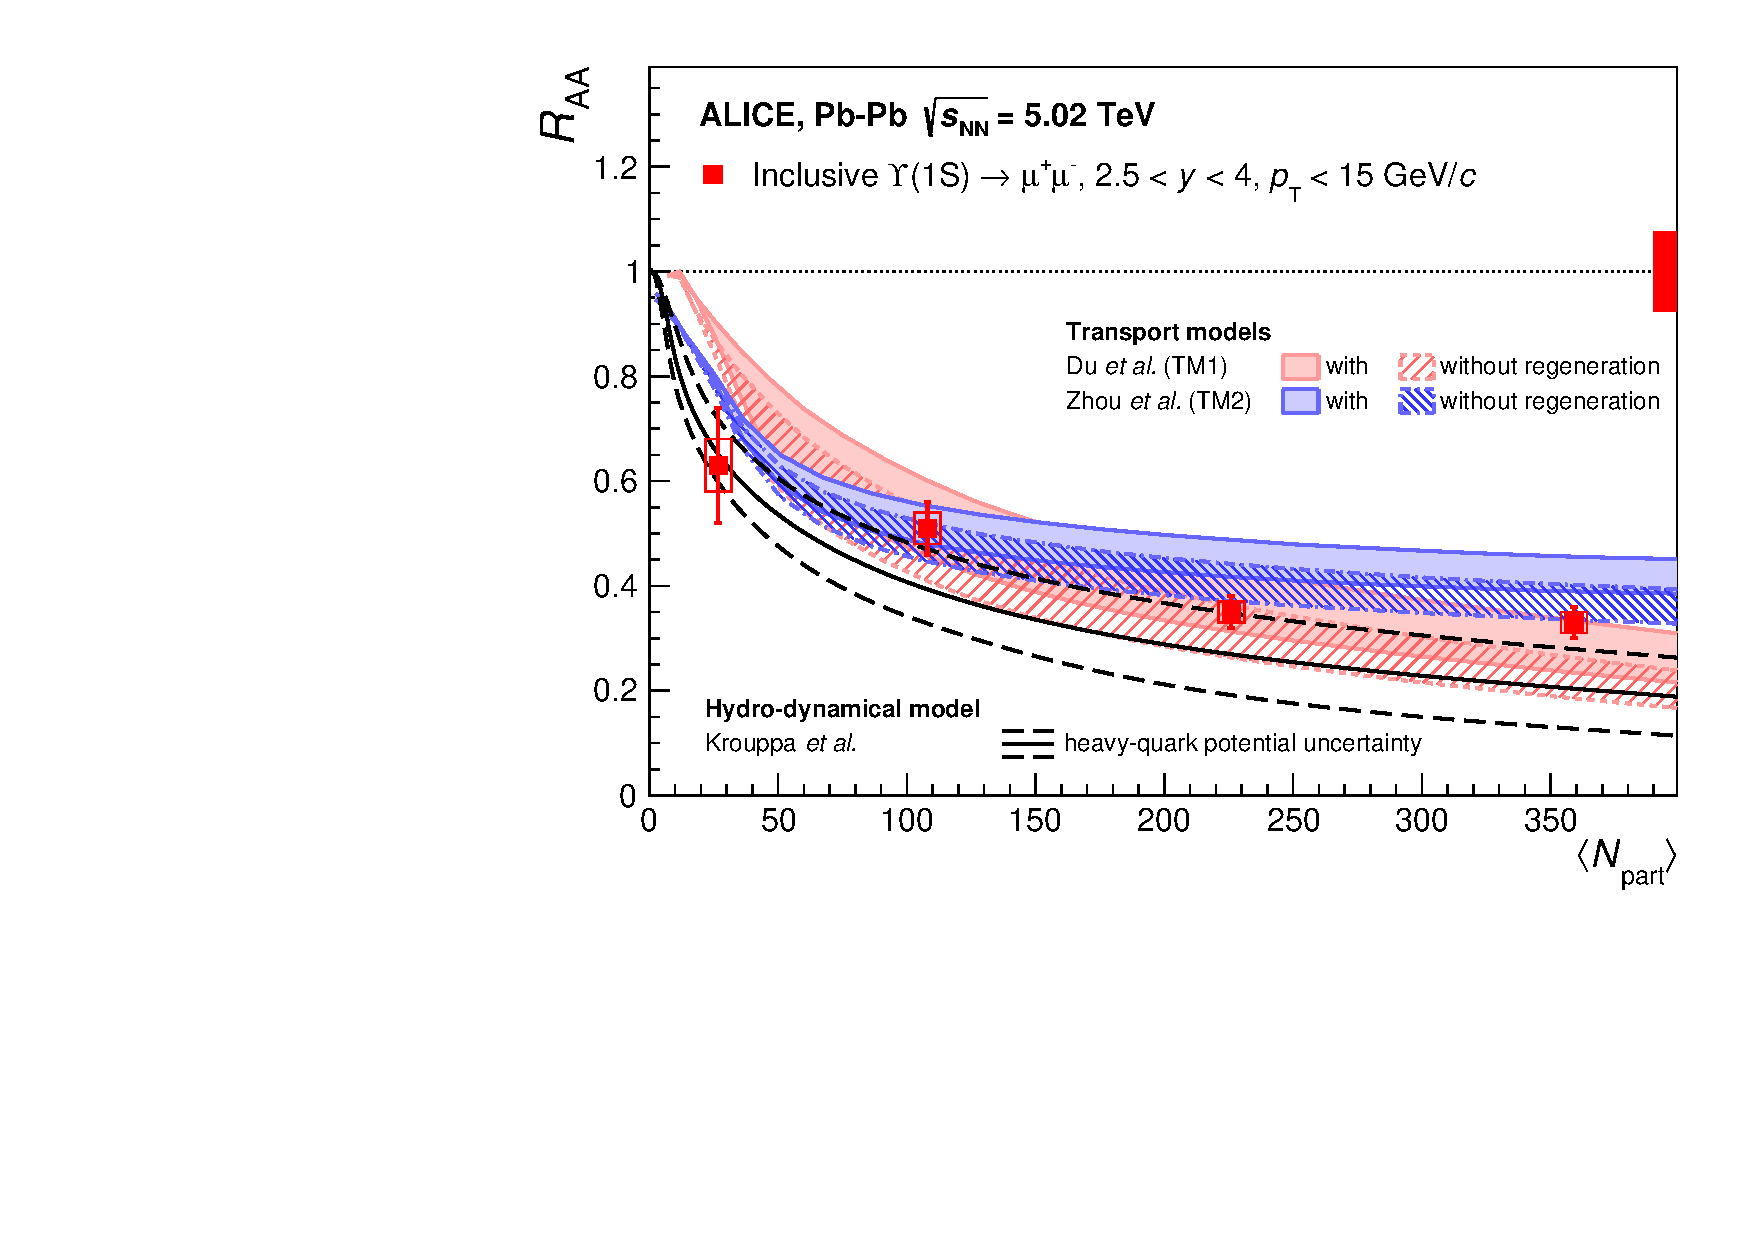
\includegraphics[width=0.5\linewidth]{Chapters/Analysis/Figs/RAA_Cent_ALICE2015_Rapp_Zhou_Strickland_style3.pdf} \\
\end{center}
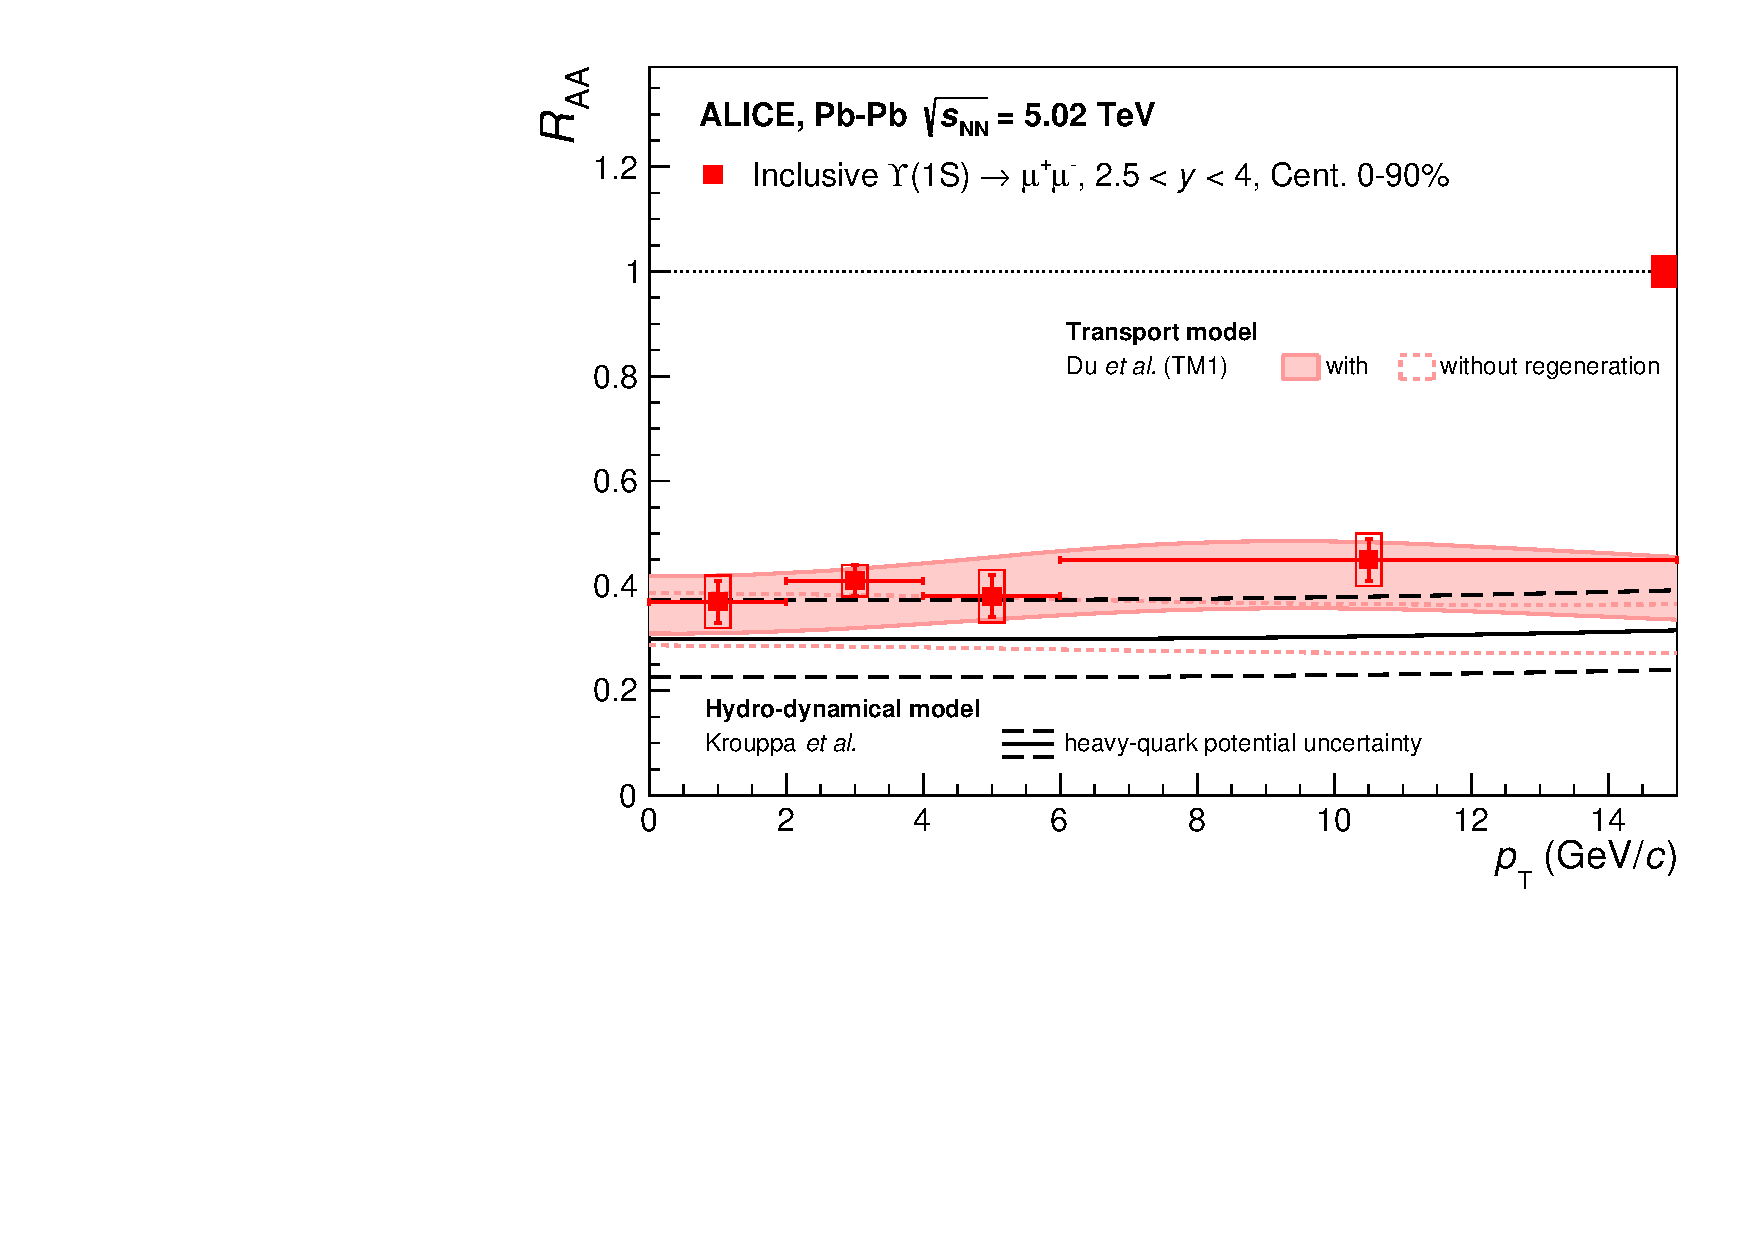
\includegraphics[width=0.5\linewidth]{Chapters/Analysis/Figs/RAA_Pt_ALICE2015_Rapp_Strickland_style3.pdf}
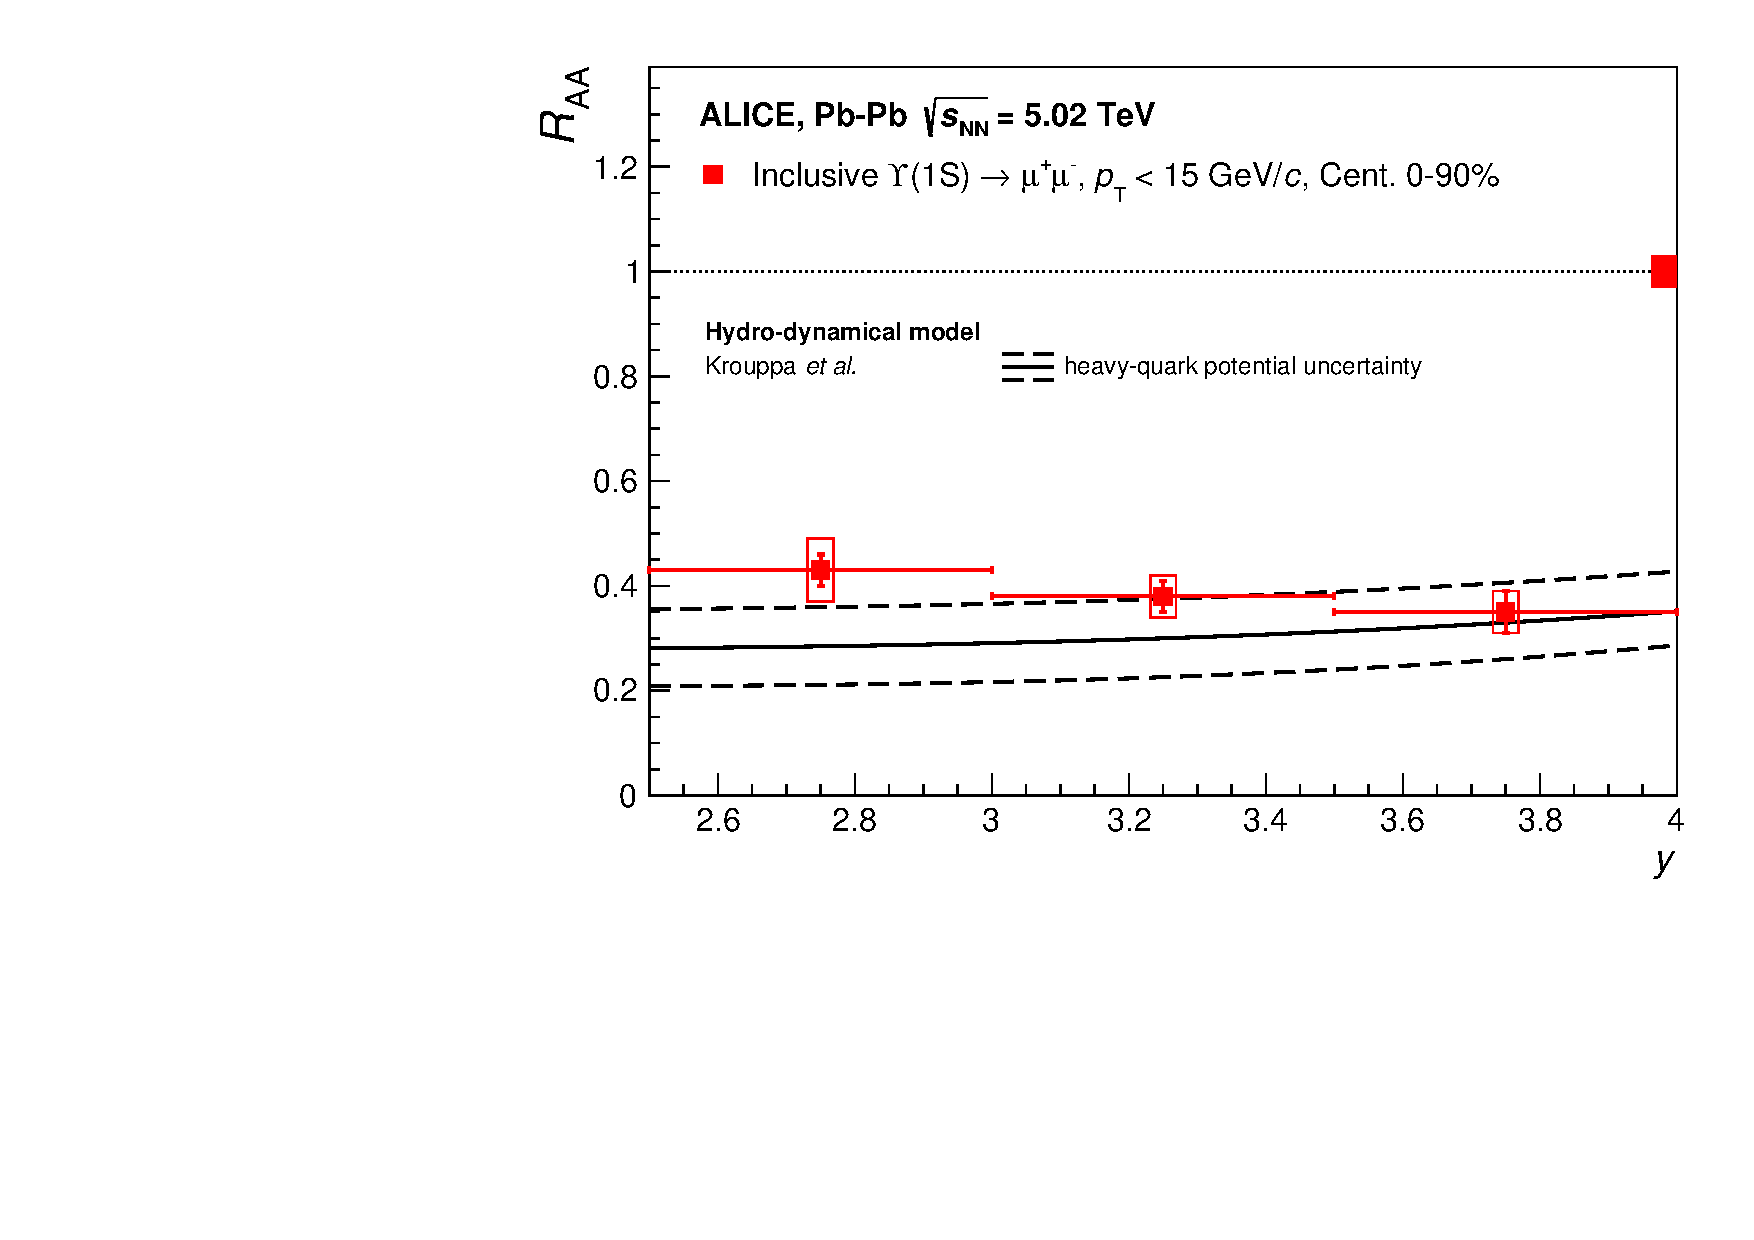
\includegraphics[width=0.5\linewidth]{Chapters/Analysis/Figs/RAA_Y_ALICE2015_Strickland_style3.pdf}
\caption{Inclusive $\upsis$ $\raa$ compared to predictions from two transport models \cite{Du:2017qkv,Zhou:2014hwa} and one hydro-dynamical model \cite{Krouppa:2017jlg} as a function of centrality (top), $\pt$ (left) and $y$ (right). See text for details on the models. While all models provide centrality dependence predictions, some of them do not provide $p_{\mathrm{T}}$ and/or $y$ estimations. The plots report all the available information at the moment of writing.}
\label{fig:raa_models}
\end{figure}

%%%%%%%%%%%%%%%%%%%%%%%%%%%%%%%%%%%%%%%%%%%%%%%%
\section{Summary}

The nuclear modification factors of inclusive \upsis and \upsiss production was measured with the ALICE detector at forward rapidity ($2.5<y<4.0$) and for $p_{\rm T}<15$ GeV/$c$ in \pbpb collisions at $\sqrt{s_{_{\rm NN}}}=5.02$~\rm{TeV}.

% The computation of double ratios between \upsis and \upsiss $\raa$ at $\sqrt{s_{_{\rm NN}}}=5.02$~\rm{TeV} and between \upsis $\raa$ at $\sqrt{s_{_{\rm NN}}}=2.76$~\rm{TeV} and $\sqrt{s_{_{\rm NN}}}=5.02$~\rm{TeV}.
The double ratio of the \upsis and \upsiss \raa was computed as well. 
The observed value of $ 0.28 \pm 0.12(stat.) \pm 0.06(syst.)$ is compatible with the hypothesis of a larger suppression for the higher-energy (more weakly bound) states.

Finally, the double ratio of the \upsi \raa measured in Pb-Pb collisions at $\sqrt{s_{_{\rm NN}}}=5.02$ and $2.76$~\rm{TeV} was computed as well. 
The result shows no significant energy dependence at the LHC.

% The ratio between \upsis and \upsiss productions is aligned  with the hypothesis of a binding-energy dependent sequential suppression, given the higher energy state is clearly more suppressed than the fundamental one.
% The ratio computed for \upsis at different energies, however, showed no significant energy hierarchy at the LHC energies.
% Even if no clear hint on an energy dependence of the suppression/recombination mechanisms at the LHC energies is present, from the comparison between ALICE results at the LHC and previous results at RHIC a symmetry between $J/\psi$ at RHIC and \upsis at the LHC can be noticed.
% This observation can suggest that a recombination mechanism similar to the one observed for $J/\psi$ at RHIC can be present for \upsis at the LHC.
% That can eventually be in agreement with the estimation of the average number of produced $c-\bar{c}$ and $b-\bar{b}$ pairs at the two accelerators energies.

The results have been compared with transport and hydrodynamic models.
The transport models are able to provide prediction with and without including recombination effects.
The comparison between the measurements with the different predictions lead to no clear conclusion on whether recombination effects play a role.
Further measurements with larger statistics will be needed to improve the precision and to better constrain the models.